\chapter{Mechanism and Structure Schematics}

\makeatletter
\@ifundefined{chsevenrelmark}{%
\newcommand{\chsevenrelmark}[2][]{%
  \tikz[baseline=(char.base)]{%
    \node[shape=circle, draw=BookInk, line width=0.5pt, fill=white, inner sep=1pt,
      font=\sffamily\fontsize{6.5}{6.5}\selectfont, #1] (char)
      {\@ifundefined{chseven@num@#2}{#2}{\csname chseven@num@#2\endcsname}};}}%
}{}
\definecolor{ch07err}{HTML}{C0392B}
\@ifundefined{chsevenerrmark}{%
\newcommand{\chsevenerrmark}[2][]{%
  \tikz[baseline=(char.base)]{%
    \node[shape=circle, fill=ch07err, text=white, inner sep=1.5pt,
      font=\sffamily\fontsize{7}{7}\selectfont\bfseries, #1] (char)
      {\@ifundefined{chseven@num@#2}{#2}{\csname chseven@num@#2\endcsname}};}}%
}{}
\@ifundefined{chsevenpanelbase}{%
  \newcommand{\chsevenpanelbase}{figures/ch07/ch07-08-battery-base.png}%
}{}
\@ifundefined{chsevendrawcircuit}{%
\newcommand{\chsevendrawcircuit}[1]{%
  \def\ChSevenWireY{1.10}%
  \def\ChSevenTabY{0.878}%
  \draw[ch07wire, line width=0.8pt] (0.194, \ChSevenTabY) -- (0.194, \ChSevenWireY);
  \draw[ch07wire, line width=0.8pt] (0.805, \ChSevenTabY) -- (0.805, \ChSevenWireY);
  \draw[ch07wire, line width=0.8pt] (0.194, \ChSevenWireY) -- (0.805, \ChSevenWireY);
  \node[draw=ch07wire, line width=0.6pt, rounded corners=1.5pt, fill=white,
    font=\sffamily\scriptsize, inner sep=1.6pt]
    at (0.50, \ChSevenWireY) {#1};
  \foreach \chyy in {0.38, 0.52, 0.66} {%
    \draw[-{Stealth[length=2mm]}, ch07Li, line width=0.9pt]
      (0.68, 1-\chyy) -- (0.32, 1-\chyy);
  }%
  \node[font=\sffamily\scriptsize, text=ch07Li, fill=white, inner sep=0.7pt]
    at (0.50, 1-0.30) {Li\textsuperscript{+}};
  \draw[ch07elec, line width=0.7pt, dashed, -{Stealth[length=1.5mm]}]
    (0.76, \ChSevenWireY) -- (0.62, \ChSevenWireY);
  \draw[ch07elec, line width=0.7pt, dashed, -{Stealth[length=1.5mm]}]
    (0.38, \ChSevenWireY) -- (0.24, \ChSevenWireY);
}%
}{}
\@ifundefined{chsevendrawcircuitb}{%
\newcommand{\chsevendrawcircuitb}[1]{%
  \def\ChSevenWireY{1.10}%
  \def\ChSevenTabY{0.878}%
  \draw[ch07wire, line width=0.8pt] (0.194, \ChSevenTabY) -- (0.194, \ChSevenWireY);
  \draw[ch07wire, line width=0.8pt] (0.805, \ChSevenTabY) -- (0.805, \ChSevenWireY);
  \draw[ch07wire, line width=0.8pt] (0.194, \ChSevenWireY) -- (0.805, \ChSevenWireY);
  \node[draw=ch07wire, line width=0.6pt, rounded corners=1.5pt, fill=white,
    font=\sffamily\scriptsize, inner sep=1.6pt]
    at (0.50, \ChSevenWireY) {#1};
  \foreach \chyy in {0.38, 0.52, 0.66} {%
    \draw[-{Stealth[length=2mm]}, ch07Li, line width=0.9pt]
      (0.32, 1-\chyy) -- (0.68, 1-\chyy);
  }%
  \node[font=\sffamily\scriptsize, text=ch07Li, fill=white, inner sep=0.7pt]
    at (0.50, 1-0.30) {Li\textsuperscript{+}};
  \draw[ch07elec, line width=0.7pt, dashed, -{Stealth[length=1.5mm]}]
    (0.24, \ChSevenWireY) -- (0.38, \ChSevenWireY);
  \draw[ch07elec, line width=0.7pt, dashed, -{Stealth[length=1.5mm]}]
    (0.62, \ChSevenWireY) -- (0.76, \ChSevenWireY);
}%
}{}
\makeatother

While drafting a manuscript on insulin resistance in skeletal muscle, a graduate student named Zhou wanted an opening schematic (Figure 1) to summarize the canonical pathway by which insulin promotes the translocation of glucose transporter 4 (GLUT4) to the cell surface. She opened an image generator and typed a single sentence: ``Make a beautiful, professional scientific illustration of insulin signaling and GLUT4 translocation for a top journal.'' Within a minute, a striking image appeared: glossy three-dimensional proteins floated across a deep indigo cellular interior, golden phosphorylation orbs glowed along white arrows, and a detailed nucleus, rough endoplasmic reticulum, Golgi apparatus, and microtubule bundle filled the corners. Convinced that the artwork looked far more polished than anything she could assemble in a vector editor, she placed it straight into her draft.

At lab meeting, her advisor and a senior postdoc needed less than three minutes to find four fatal flaws. First, the arrow from the serine/threonine kinase Akt to its substrate AS160 was drawn as a solid white activation arrow, whereas Akt actually phosphorylates and \emph{inhibits} the GTPase-activating protein (GAP) activity of AS160. Second, the mammalian target of rapamycin complex 2 (mTORC2) branch required for full Akt activation was completely missing. Third, the small GTPase Rab floated freely in the cytosol instead of associating with the storage vesicles it regulates. Fourth, ligand binding, lipid conversion, kinase phosphorylation, vesicle trafficking, and transmembrane glucose uptake all used the exact same solid white arrowhead, leaving readers unable to tell chemical catalysis from physical movement.

When peer reviewers critique a mechanism diagram or a device cross-section, they are not grading specular highlights, ambient occlusion, or decorative organelles; they are checking whether every visual link states a defensible scientific proposition. A mechanism schematic depicts causal and spatial relations rather than a list of nouns, and a structural schematic depicts layer sequence, material pairing, and transport direction under a defined operating state. Whenever a prompt omits an explicit relation table, line-style dictionary, and compartment layout, a generative model bridges the gaps with plausible-looking visual guesswork. Using two complete cases---a cell-signaling pathway from metabolism and a pouch-cell cross-section from electrochemistry---this chapter shows how to decompose established domain knowledge into verifiable tables, generate clean text-free base artwork with AI, and finish the figure by overlaying exact typography, circuit symbols, and legends in LaTeX/TikZ.

\section{What a Mechanism Figure Must State}

Before writing a prompt or touching a canvas, an author must decide what propositions a mechanism figure needs to communicate. Across disciplines---whether intracellular signal transduction, heterogeneous catalysis, or contaminant transformation across environmental interfaces---a rigorous mechanism schematic must state four things: objects, compartments, interactions, and evidence status (Figure~\ref{fig:ch07-01}).

\begin{figure}[htbp]\centering
% FIG ch07-01 mechanism grammar (English labels)
\begin{tikzpicture}[
  font=\sffamily\small,
  paneltitle/.style={font=\sffamily\bfseries\footnotesize, text=BookInk, anchor=west},
  foot/.style={font=\sffamily\scriptsize, text=BookInk!80},
  infobox/.style={
    draw=BookRule, line width=0.6pt, rounded corners=2pt, fill=BookPale,
    font=\sffamily\scriptsize, align=center,
    text width=48mm, minimum height=9mm, inner sep=2.6pt
  },
  band/.style={
    draw=BookRule, line width=0.5pt,
    font=\sffamily\scriptsize, align=left,
    text width=48mm, minimum height=6.4mm, inner sep=2.4pt
  },
  evbox/.style={
    draw=BookRule, line width=0.5pt, fill=BookPale,
    font=\sffamily\scriptsize, align=left,
    text width=48mm, minimum height=13mm, inner sep=2.6pt
  },
]
\definecolor{ch07act}{HTML}{3A3A3A}
\definecolor{ch07conv}{HTML}{7A7A7A}
\definecolor{ch07trans}{HTML}{E39B5B}
\definecolor{ch07flux}{HTML}{C46A2A}
\definecolor{ch07phos}{HTML}{E3B23C}
\definecolor{ch07hyp}{HTML}{9A9A9A}

\node[paneltitle] (tObj) at (0,0) {Objects};
\node[infobox, anchor=north west] (bObj) at ([yshift=-1.2mm]tObj.south west) {What they are\\how often};

\node[paneltitle, anchor=north west] (tComp) at ([yshift=-3.2mm]bObj.south west) {Compartments};
\node[band, fill=BookPale!50, anchor=north west] (bExt) at ([yshift=-1.2mm]tComp.south west) {Extracellular};
\node[band, fill=white, anchor=north west] (bMem) at ([yshift=-1.1mm]bExt.south west) {Membrane};
\node[band, fill=BookPale!30, anchor=north west] (bCyt) at ([yshift=-1.1mm]bMem.south west) {Cytoplasm};

\node[paneltitle, anchor=north west] (tInt) at ([yshift=-3.2mm]bCyt.south west) {Interactions};
\node[band, fill=BookPale, minimum height=7.2mm, align=center, anchor=north west]
  (bInt) at ([yshift=-1.2mm]tInt.south west)
  {\tikz[baseline=-0.55ex]{\draw[-{Stealth[length=2mm]}, ch07act, line width=0.8pt] (0,0) -- (32mm,0);}};

\node[paneltitle, anchor=north west] (tEv) at ([yshift=-3.2mm]bInt.south west) {Evidence};
\node[evbox, anchor=north west] (bEv) at ([yshift=-1.2mm]tEv.south west) {%
  \begin{tabular}{@{}l@{\hspace{1.8mm}}l@{}}
    \tikz[baseline=-0.55ex]{\draw[ch07act, line width=0.8pt] (0,0) -- (16mm,0);} & Established \\[1.4mm]
    \tikz[baseline=-0.55ex]{\draw[ch07hyp, line width=0.8pt, dashed] (0,0) -- (16mm,0);} & Hypothesis
  \end{tabular}};

\node[paneltitle] (rt) at (60mm,0) {Line conventions (this chapter)};
\draw[-{Stealth[length=2mm]}, ch07act, line width=0.8pt] (60mm,-8mm) -- (78mm,-8mm);
\node[anchor=west, font=\sffamily\small] at (82mm,-8mm) {Activation};
\draw[-{Bar[width=6pt]}, ch07act, line width=0.8pt] (60mm,-15.5mm) -- (78mm,-15.5mm);
\node[anchor=west, font=\sffamily\small] at (82mm,-15.5mm) {Inhibition};
\draw[ch07conv, line width=0.5pt] (60mm,-23mm) .. controls (66mm,-21.2mm) and (72mm,-24.8mm) .. (76mm,-23mm);
\draw[-{Straight Barb[open]}, ch07conv, line width=0.5pt] (76mm,-23mm) -- (78mm,-23mm);
\node[anchor=west, font=\sffamily\small] at (82mm,-23mm) {Enzymatic conversion};
\draw[ch07trans, line width=1.5pt, dashed, -{Stealth[length=2.5mm, open]}] (60mm,-30.5mm) -- (78mm,-30.5mm);
\node[anchor=west, font=\sffamily\small] at (82mm,-30.5mm) {Vesicle translocation};
\draw[ch07flux, line width=0.8pt, dotted, -{Stealth[length=2mm]}] (60mm,-38mm) -- (78mm,-38mm);
\node[anchor=west, font=\sffamily\small] at (82mm,-38mm) {Glucose flux};
\draw[ch07hyp, line width=0.8pt, dashed, -{Stealth[length=2mm]}] (60mm,-45.5mm) -- (78mm,-45.5mm);
\node[anchor=west, font=\sffamily\small] at (82mm,-45.5mm) {Hypothesised link};
\fill[ch07phos] (62mm,-53mm) circle (2pt);
\node[anchor=west, font=\sffamily\small] at (82mm,-53mm) {Phosphorylation (amber dot)};
\node[anchor=north west, font=\sffamily\scriptsize, text=BookInk!70, align=left, text width=68mm]
  at (60mm,-58mm) {Figure~1 example has no hypothesised links};

\node[foot, anchor=north west] at ([yshift=-3mm]current bounding box.south west)
  {Legend defines line meaning; field conventions (e.g.\ SBGN) inform the choices.};
\end{tikzpicture}

\caption{The four kinds of information a mechanism figure must state, and the line conventions used in this chapter. Each relation type gets exactly one line style, and hypothesised links must be distinguishable from established ones. The legend, informed by field conventions, defines what each line means.}\label{fig:ch07-01}
\end{figure}

\textbf{First, objects: what each entity is and how many times it appears.} Every shape in a schematic represents a conceptual entity---a ligand, transmembrane receptor, intracellular kinase, membrane lipid, or storage vesicle. When the same molecule appears twice in one diagram, a reader naturally asks whether the duplication represents two subunits, two conformational states, or two locations before and after transport. Without strict multiplicity rules, image models routinely duplicate icons to fill space, such as lining up six identical transporter barrels in one membrane pit. An object inventory must therefore specify both identity and count. Any node acting at a single step (the insulin receptor, IRS-1, PI3K, PDK1, Akt, mTORC2, AS160) should appear once. Only when the mechanism involves spatial relocation may an object appear twice: GLUT4 is shown once embedded in intracellular storage vesicles (reserve state) and once inserted into the plasma membrane (active state), drawn with identical geometry and colour.

Object design also requires only ``necessary structural detail.'' A pathway schematic clarifies causal logic rather than atomic structure. Include only morphological features that affect mechanistic understanding: the insulin receptor must span the bilayer to transmit an extracellular signal indoors, and Rab must sit on the storage vesicle surface where it acts. By contrast, drawing the disulfide-linked $\alpha_2\beta_2$ tetramer details of the insulin receptor or the p85/p110 subunit interface of PI3K adds clutter and invites model distortion; such features are better simplified into clean silhouettes and noted in the caption.

\textbf{Second, compartments: spatial partitioning is itself scientific information.} Treating membranes, phase boundaries, or organelles as decorative backdrops is a primary source of localization error. In insulin signaling, insulin remains in the extracellular space contacting the receptor ectodomain; phosphatidylinositol 4,5-bisphosphate ($\text{PIP}_2$) and 3,4,5-trisphosphate ($\text{PIP}_3$) are anchored in the inner leaflet of the plasma membrane rather than floating in the cytosol; and PDK1 and Akt must bind inner-leaflet $\text{PIP}_3$ via their PH domains to be activated, so both belong directly against the cytoplasmic face of the membrane. Dividing the canvas into explicit zones---extracellular space, plasma membrane, and cytoplasm---turns two-dimensional coordinates into a verifiable statement of subcellular localization.

\textbf{Third, interactions: assign exactly one line style to each relation type.} Many drafts suffer from arrow overloading, using one solid arrow for kinase phosphorylation, lipid conversion, vesicle movement, and transmembrane flux alike. When distinct processes share one symbol, readers must guess the mechanism; worse, using a pointed arrowhead for an inhibitory step turns negative regulation into activation.

The core principle of the Systems Biology Graphical Notation (SBGN; Le Nov\`ere et al., 2009; see also the official SBGN website) is to assign each interaction class a mutually exclusive glyph. Without adopting the full engineering syntax of SBGN, authors should establish a self-consistent line dictionary within every figure. Our main case study distinguishes five interaction styles and one state marker (Figure~\ref{fig:ch07-01}, right):
\begin{itemize}
\item \textbf{Direct binding and membrane recruitment:} Geometric contact without an arrow (insulin touching the receptor top; PDK1 and Akt touching the inner leaflet at $\text{PIP}_3$), reducing arrow clutter.
\item \textbf{Activation or stimulation:} Solid dark-grey line with a filled triangular head for positive regulation between signaling proteins.
\item \textbf{Inhibition:} Solid dark-grey line of the same weight ending in a perpendicular flat bar (T-bar) touching the target outline.
\item \textbf{Enzymatic chemical conversion:} Thinner mid-grey curved arc with an open V head from substrate to product, met at its midpoint by a short stub from the enzyme.
\item \textbf{Spatial translocation:} Thick dashed soft-orange arrow with a large open head representing physical movement of vesicles to the membrane.
\item \textbf{Transmembrane substance flux:} Dotted dark-orange line with a small filled head passing through the transporter channel to show glucose influx.
\item \textbf{Phosphorylation state:} Small amber dots on phosphorylated proteins rather than baked-in ``P'' letters, defined in the legend.
\end{itemize}

No line style has universal meaning outside its context. Because conventions vary across fields, every schematic must include an on-canvas legend and restate the definitions in the caption.

\textbf{Fourth, evidence status: separate established consensus, readability simplifications, and working hypotheses.} Mechanism figures often mix textbook facts, deliberate omissions for legibility, and newly proposed hypotheses. Drawing all three as identical solid lines invites reviewers to fault the figure for overstating speculation or omitting known branches. Instead, draw consensus steps as solid lines, declare omitted isoforms or parallel branches in the caption, and render hypothetical links as mid-grey dashed arrows labelled ``Hypothesised link'' in both legend and caption.

\section{From Relation Table to Sketch}

With these four requirements set, the next step is not to write an English prompt directly, but to organize the source material into a relation table as introduced in Chapter 2. We illustrate this using the canonical insulin-stimulated GLUT4 translocation pathway in skeletal muscle or adipose cells.

Suppose we are preparing Figure 1 of a paper to orient peers to this classic pathway. The figure reports no new data or hypotheses; every link rests on established reviews and primary studies (Saltiel and Kahn, 2001; Leto and Saltiel, 2012; Klip et al., 2019; Sano et al., 2003 for AS160; Sarbassov et al., 2005 for mTORC2). Listing thirteen protein names alone tells neither a human nor an AI who acts upstream or who inhibits whom. Writing them as the thirteen rows (R1--R13) of Table~\ref{tab:ch07-01} fixes every source, target, line style, compartment, and simplification.

\begin{table}[htbp]\centering\scriptsize
\setlength{\tabcolsep}{3pt}
\renewcommand{\arraystretch}{0.95}
\caption{Relation table (R1--R13) for insulin-stimulated GLUT4 translocation. Each row corresponds to one contact or connecting line in the figure.}\label{tab:ch07-01}
\begin{tabularx}{\linewidth}{lYYYYY}
\toprule
\textbf{ID} & \textbf{Source} & \textbf{Target / outcome} & \textbf{Relation \& line style} & \textbf{Compartment} & \textbf{Status \& simplification} \\
\midrule
R1 & Insulin & Insulin receptor (IR) & Binding (direct contact, no arrow) & Extracellular / outer membrane & Established; transmembrane dimer outline, omit $\alpha_2\beta_2$ details \\
R2 & Bound IR & IR kinase domain & Auto-phosphorylation (2 amber dots) & Cytoplasmic face of membrane & Established; omit specific Tyr residue numbers \\
R3 & Active IR & IRS-1 & Phosphorylation activation (solid arrow + 1 dot) & Sub-membrane cytoplasm & Established; IRS-1/2 both act in muscle/fat, show IRS-1 only \\
R4 & Phospho-IRS-1 & Class IA PI3K & Recruitment \& activation (solid arrow) & Sub-membrane cytoplasm & Established; do not split p85 and p110 subunits \\
R5 & PI3K & $\text{PIP}_2 \rightarrow \text{PIP}_3$ & Enzymatic conversion (thin arc, open V head, PI3K stub at midpoint) & Inner leaflet of membrane & Established; omit PTEN and SHIP2 dephosphorylation \\
R6 & $\text{PIP}_3$ & PDK1 and Akt & Membrane recruitment (touch inner leaflet, no arrow) & Inner leaflet of membrane & Established; omit PH domain, express by membrane contact \\
R7 & PDK1 & Akt & Thr308 phosphorylation (solid arrow) & Inner face of membrane & Established; shares 2 amber dots on Akt with R8 \\
R8 & mTORC2 & Akt & Ser473 phosphorylation (solid arrow) & Sub-membrane cytoplasm & Established (Sarbassov et al., 2005); no upstream arrow into mTORC2 \\
R9 & Active Akt & AS160 (TBC1D4) & Phosphorylation \& GAP inhibition (T-bar + 1 dot) & Cytoplasm & Established (Sano et al., 2003); omit 14-3-3 and TBC1D1 \\
R10 & AS160 & Vesicle Rab & Inhibition of Rab activity (T-bar touching Rab) & Storage vesicle surface & Established; do not distinguish Rab8A/10/13 isoforms \\
R11 & Rab-GTP & GLUT4 storage vesicles (GSVs) & Promotion of translocation (thick dashed orange arrow, open head) & Cytoplasm $\rightarrow$ membrane & Established; omit microtubules, actin, and motor proteins \\
R12 & Translocated GSVs & Membrane GLUT4 & Membrane fusion \& insertion (dashed arrow ends at membrane GLUT4) & Plasma membrane & Established; omit VAMP2/syntaxin-4 SNARE proteins \\
R13 & Extracellular glucose & Intracellular glucose & Facilitated diffusion via GLUT4 (dotted dark-orange arrow downward) & Extracellular $\rightarrow$ cytoplasm & Established; omit hexokinase and downstream glycolysis \\
\bottomrule
\end{tabularx}
\end{table}

Below the table we also record an explicit exclusion list of what not to draw: the Grb2--SOS--Ras--MAPK mitogenic branch; the debated CAP--Cbl--TC10 branch; GLUT4 endocytosis and recycling; S6K negative feedback and contraction-activated AMPK signaling (Leto and Saltiel, 2012; Klip et al., 2019); and any quantitative data. Stating what to omit both constrains the AI prompt and prepares the simplification disclosure in the figure legend.

From Table~\ref{tab:ch07-01}, five minutes with a pencil yields a layout sketch (V0) placing all thirteen relations into two-dimensional space (Figure~\ref{fig:ch07-02}). A sketch fixes only compartments and reading order: a horizontal double line across the top fifth represents the plasma membrane, separating extracellular space, membrane, and cytoplasm. The main cascade runs left to right just below the membrane from the receptor to Akt, steps down and right via two consecutive T-bars to the vesicle cluster, and curves upward via a thick dashed arrow to the membrane GLUT4 beneath the downward dotted glucose line---forming a ``left $\rightarrow$ right, then lower-right $\rightarrow$ upper-right'' trajectory while reserving the bottom tenth for a legend.

\begin{figure}[htbp]\centering
% FIG ch07-02 relation-number overlay (language-neutral)
\makeatletter
\@ifundefined{chsevenrelmark}{%
\newcommand{\chsevenrelmark}[2][]{%
  \tikz[baseline=(char.base)]{%
    \node[shape=circle, draw=BookInk, line width=0.5pt, fill=white, inner sep=1pt,
      font=\fontsize{7}{7}\selectfont, #1] (char) {#2};}}%
}{}
\makeatother
\begin{tikzpicture}
  \node[anchor=south west, inner sep=0] (img) at (0,0)
    {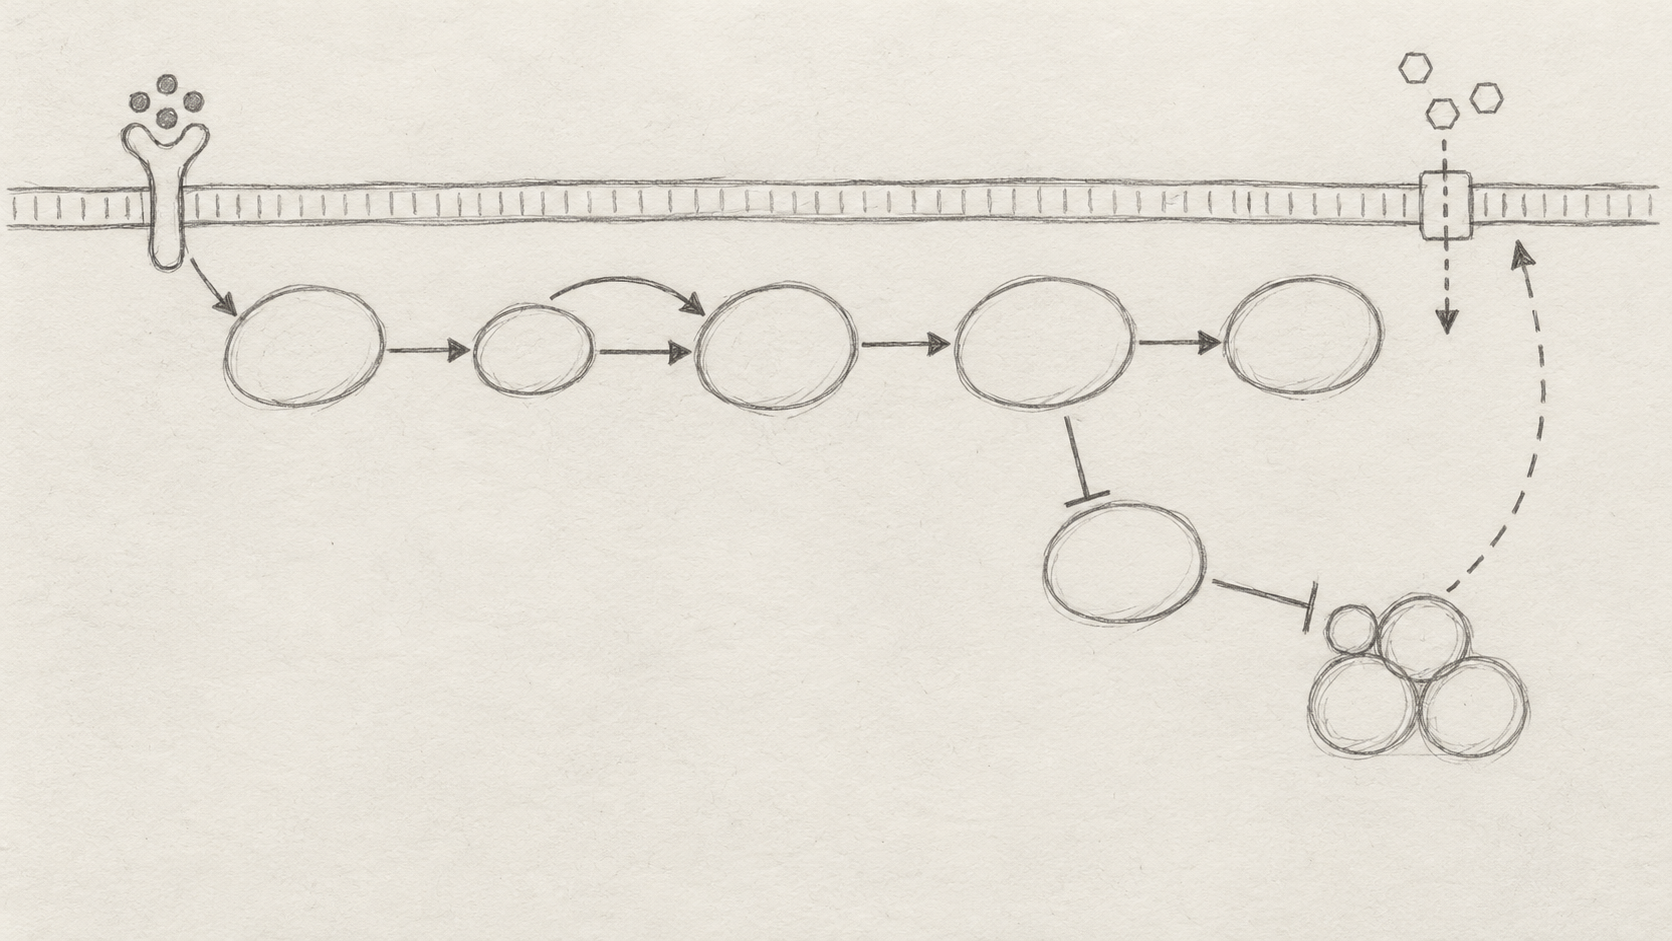
\includegraphics[width=\linewidth]{figures/ch07/ch07-02-v0-sketch.png}};
  \begin{scope}[x={(img.south east)}, y={(img.north west)}]
    \node at (0.12, 1-0.10) {\chsevenrelmark{1}};
    \node at (0.12, 1-0.28) {\chsevenrelmark{2}};
    \node at (0.17, 1-0.44) {\chsevenrelmark{3}};
    \node at (0.25, 1-0.42) {\chsevenrelmark{4}};
    \node at (0.37, 1-0.26) {\chsevenrelmark{5}};
    \node at (0.47, 1-0.37) {\chsevenrelmark{7}};
    \node at (0.53, 1-0.50) {\chsevenrelmark{8}};
    \node at (0.58, 1-0.46) {\chsevenrelmark{9}};
    \node at (0.67, 1-0.58) {\chsevenrelmark{10}};
    \node at (0.80, 1-0.45) {\chsevenrelmark{11}};
    \node at (0.87, 1-0.24) {\chsevenrelmark{12}};
    \node at (0.88, 1-0.12) {\chsevenrelmark{13}};
    \node at (0.44, 1-0.36) {\chsevenrelmark{6}};
  \end{scope}
\end{tikzpicture}

\caption{A planning sketch laid out from the relation table (a pencil sketch simulated by an image model, not a real manuscript page). Circled numbers map to relations R1--R13 in Table~\ref{tab:ch07-01}. The sketch fixes compartments, rough positions and reading order only; used as input for generation, it conveys layout intent and does not lock the layout.}\label{fig:ch07-02}
\end{figure}

The base image of Figure~\ref{fig:ch07-02} was generated by an image model simulating a pencil sketch, with circled numbers (1)--(13) overlaid in TikZ. Even for a rough sketch, running the same prompt three times exposed typical model drift: the first two runs drew only one T-bar and left the lower-right vesicle regulator disconnected from the main chain. Only on the third run---after we added an explicit instruction requiring two consecutive T-bars connecting the fourth main-chain blob to the lower-right blob and the vesicle-surface bead---did the series of (9) and (10) appear as in Figure~\ref{fig:ch07-02}. At the same time, the model dropped the upward mTORC2 blob below Akt, drew the glucose path (13) as short dashes rather than dots, and left a tiny gap between the insulin dots (1) and the receptor.

This clarifies the role of a sketch: it carries no molecular names, helping the author and tool align on compartments and flow. In \scidraw{}, an author can upload a sketch in sketch mode alongside a text brief to generate a draft, but sketch conditioning expresses layout intent rather than rigid object locking, so the output must still be checked row by row against Table~\ref{tab:ch07-01}.

\section{Why One Sentence Is Not Enough}

To see how input completeness governs scientific accuracy, we can compare the output of our opening one-sentence prompt (V1) against a draft driven by a complete figure brief (V2) under identical generation settings (Figure~\ref{fig:ch07-03}).

When working in \scidraw{}, the recommended starting point is to save a structured brief derived from your relation table in your own document, then open the Scientific Figure Workflow wizard (\sdtool{figure-workflow}), choose ``Mechanism \& workflow diagram'', and follow the route into the mechanism generator (\sdtool{mechanism-figure-generator}) or prompt drawing tool (\sdtool{ai-drawing}), pasting the brief in. Remember that the workflow wizard only lines up the tools in order; it does not verify biochemical accuracy on your behalf. The core sections of our structured figure brief read as follows (the full brief is archived in the \texttt{cases/} directory of the book repository):

\begin{Prompt}
[Purpose & Audience] Journal Figure 1 background schematic (double-column width 174 mm,
height ~100 mm) for metabolism and cell-biology readers.
[Goal] Show the signaling sequence Insulin -> IR -> IRS-1 -> PI3K -> PIP3 -> Akt, the
double inhibition Akt -| AS160 -| Rab, and the resulting GSV translocation, membrane
fusion, and glucose influx, without presenting any experimental data or new hypotheses.
[Objects & Counts] Each object appears once except GLUT4 (shown in vesicles and membrane):
Extracellular: insulin (3 beads), glucose (4 hexagons). Plasma membrane: lipid bilayer,
insulin receptor dimer, inner-leaflet PIP2 & PIP3, inserted GLUT4 (1 barrel).
Cytoplasm: IRS-1, PI3K, PDK1, Akt, mTORC2, AS160, vesicle-bound Rab, GSV cluster (3 vesicles).
Amber phosphorylation dots on IR (2), IRS-1 (1), Akt (2), and AS160 (1); no "P" letters.
[Relations & Line Styles] R1 insulin contacts IR (no arrow); R2 IR autophosphorylation;
R3 IR -> IRS-1, R4 IRS-1 -> PI3K, R7 PDK1 -> Akt, R8 mTORC2 -> Akt as solid dark-grey
activation arrows (no upstream arrow into mTORC2); R5 PI3K catalyses PIP2 -> PIP3 via thin
arc with open V head (PI3K stub at midpoint); R6 PIP3 recruits PDK1 & Akt to inner leaflet;
R9 Akt -| AS160 and R10 AS160 -| Rab as perpendicular T-bars; R11-R12 GSV translocation
to membrane GLUT4 as thick dashed orange arrow; R13 glucose influx as dotted orange arrow.
[Layout & Visuals] 16:9 landscape; top 20% extracellular, 20-28% membrane, 28-88% cytoplasm,
bottom 12% blank for legend. Flat 2D vector style on white; medium blue for signaling
proteins, grey-blue for AS160/Rab, soft orange for GLUT4/GSVs/glucose, warm grey membrane.
[Restrictions] Strictly no text, letters, or numbers in the base image; no nucleus, ER,
Golgi, cytoskeleton, MAPK or CAP-Cbl-TC10 branches, endocytosis, or decorative effects.
\end{Prompt}

For the counterexample V1, we submitted only the single vague sentence from the opening vignette:

\begin{Prompt}
Make a beautiful, professional scientific illustration of insulin signaling and
GLUT4 translocation for a top journal.
\end{Prompt}

For the brief-driven draft V2, we translated the structured brief into an explicit English image prompt specifying spatial bands (\texttt{SPACE}), the thirteen objects with their relative positions and counts (\texttt{OBJECTS}), the five mutually exclusive line styles (\texttt{RELATIONS}), and the forbidden elements (\texttt{DO NOT DRAW}), while prohibiting all text (full prompt in the \texttt{cases/} directory; key excerpt below):

\begin{Prompt}
Flat 2D scientific schematic for a journal figure, landscape 16:9, pure white
background. Clean vector style, flat fills, thin dark outlines, no gradients,
no shadows, no 3D. ABSOLUTELY NO TEXT: no letters, words, numbers, or symbols.
SPACE: Top 20% = extracellular; 20-28% = horizontal lipid bilayer membrane;
28-88% = cytoplasm; bottom 12% = empty white strip reserved for legend.
OBJECTS (each appears once; GLUT4 appears in vesicles and in plasma membrane):
1. Insulin (3 dark-blue beads touching receptor); 2. Transmembrane receptor (2 amber dots);
3. IRS-1 (1 amber dot); 4. PI3K; 5. Inner-leaflet PIP2 & PIP3; 6. PDK1 & 7. Akt
   (both touching inner leaflet at PIP3; Akt has 2 amber dots); 8. mTORC2 below Akt;
9. AS160 (gray-blue, 1 amber dot); 10. GSV cluster (3 vesicles with orange GLUT4 barrels);
11. Rab bead on vesicle; 12. GLUT4 in right plasma membrane; 13. Glucose hexagons above it.
RELATIONS (draw only these):
- Activation (solid dark-gray line, filled triangle): IR -> IRS-1 -> PI3K; PDK1 -> Akt; mTORC2 -> Akt.
- Inhibition (solid dark-gray line, perpendicular T-bar): Akt -| AS160; AS160 -| Rab.
- Enzymatic conversion (thin mid-gray arc, open V head): PIP2 -> PIP3, PI3K stub touching midpoint.
- Translocation (thick dashed orange arrow, open head): GSV cluster upward to membrane GLUT4.
- Substance flow (dotted dark-orange arrow): extracellular glucose through membrane GLUT4 into cell.
\end{Prompt}

\begin{figure}[htbp]\centering
% FIG ch07-03a V1 error markers (language-neutral)
\definecolor{ch07err}{HTML}{C0392B}
\makeatletter
\@ifundefined{chsevenerrmark}{%
\newcommand{\chsevenerrmark}[2][]{%
  \tikz[baseline=(char.base)]{%
    \node[shape=circle, fill=ch07err, text=white, inner sep=1.5pt,
      font=\fontsize{7}{7}\selectfont\bfseries, #1] (char) {#2};}}%
}{}
\makeatother
\begin{tikzpicture}
  \node[anchor=south west, inner sep=0] (img) at (0,0)
    {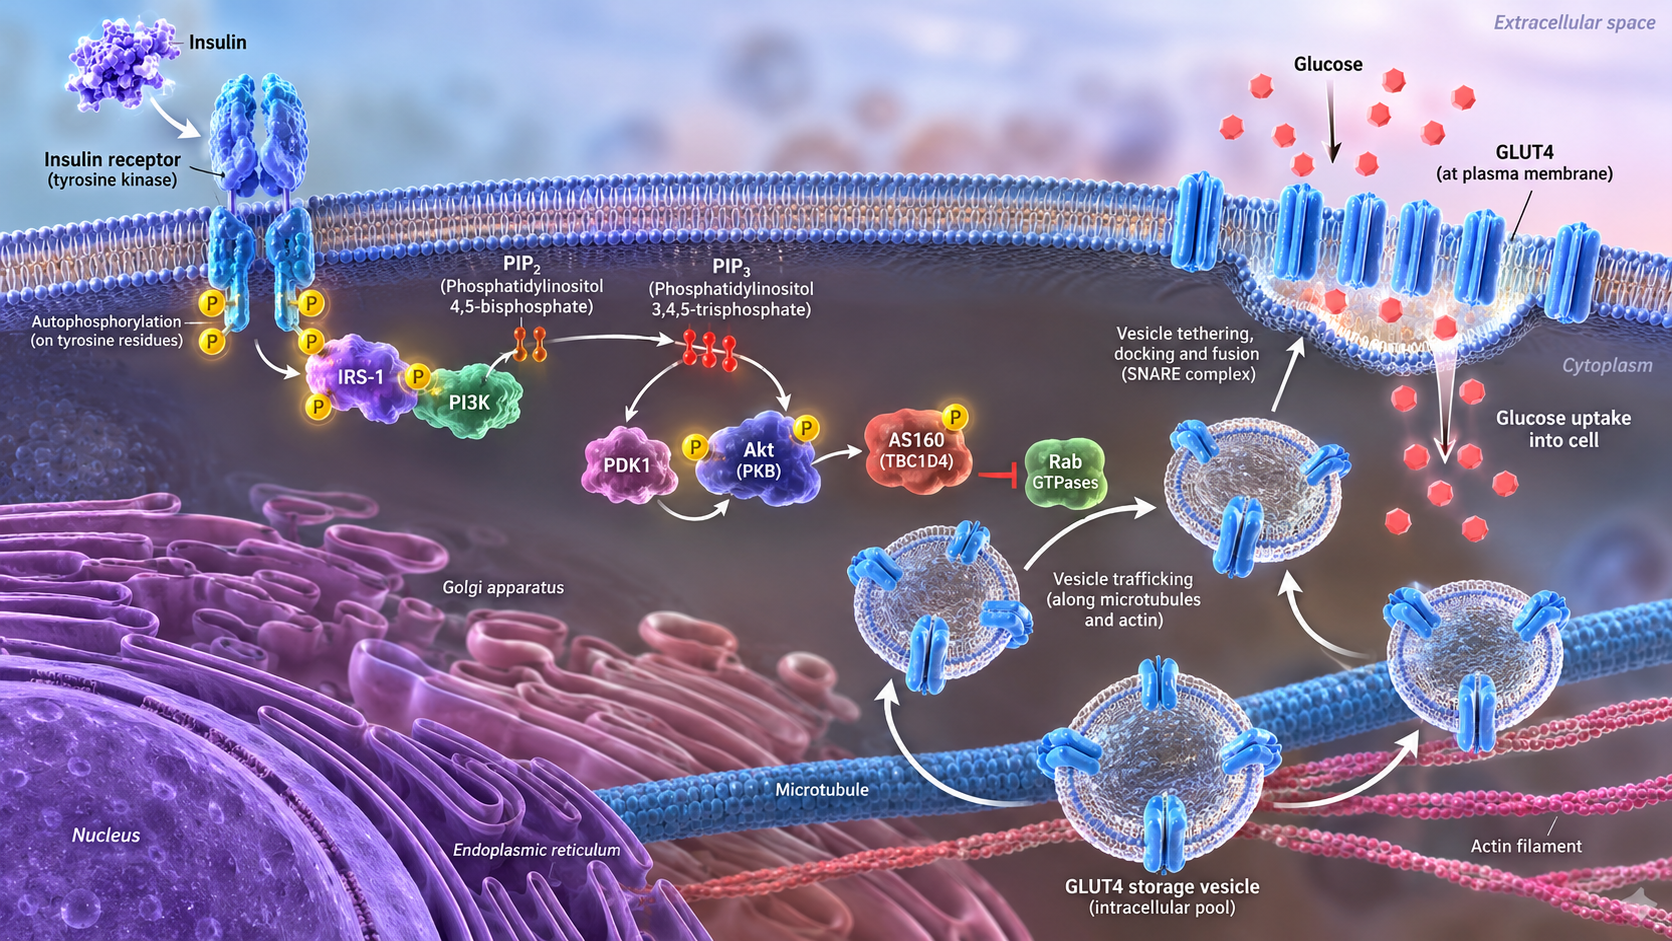
\includegraphics[width=\linewidth]{figures/ch07/ch07-03a-v1-vague.png}};
  \begin{scope}[x={(img.south east)}, y={(img.north west)}]
    \node at (0.14, 1-0.18) {\chsevenerrmark{1}};
    \node at (0.72, 1-0.22) {\chsevenerrmark{2}};
    \node at (0.50, 1-0.35) {\chsevenerrmark{3}};
    \node at (0.38, 1-0.55) {\chsevenerrmark{4}};
    \node at (0.55, 1-0.72) {\chsevenerrmark{5}};
    \node at (0.22, 1-0.48) {\chsevenerrmark{6}};
    \node at (0.82, 1-0.40) {\chsevenerrmark{7}};
  \end{scope}
\end{tikzpicture}


\vspace{2mm}
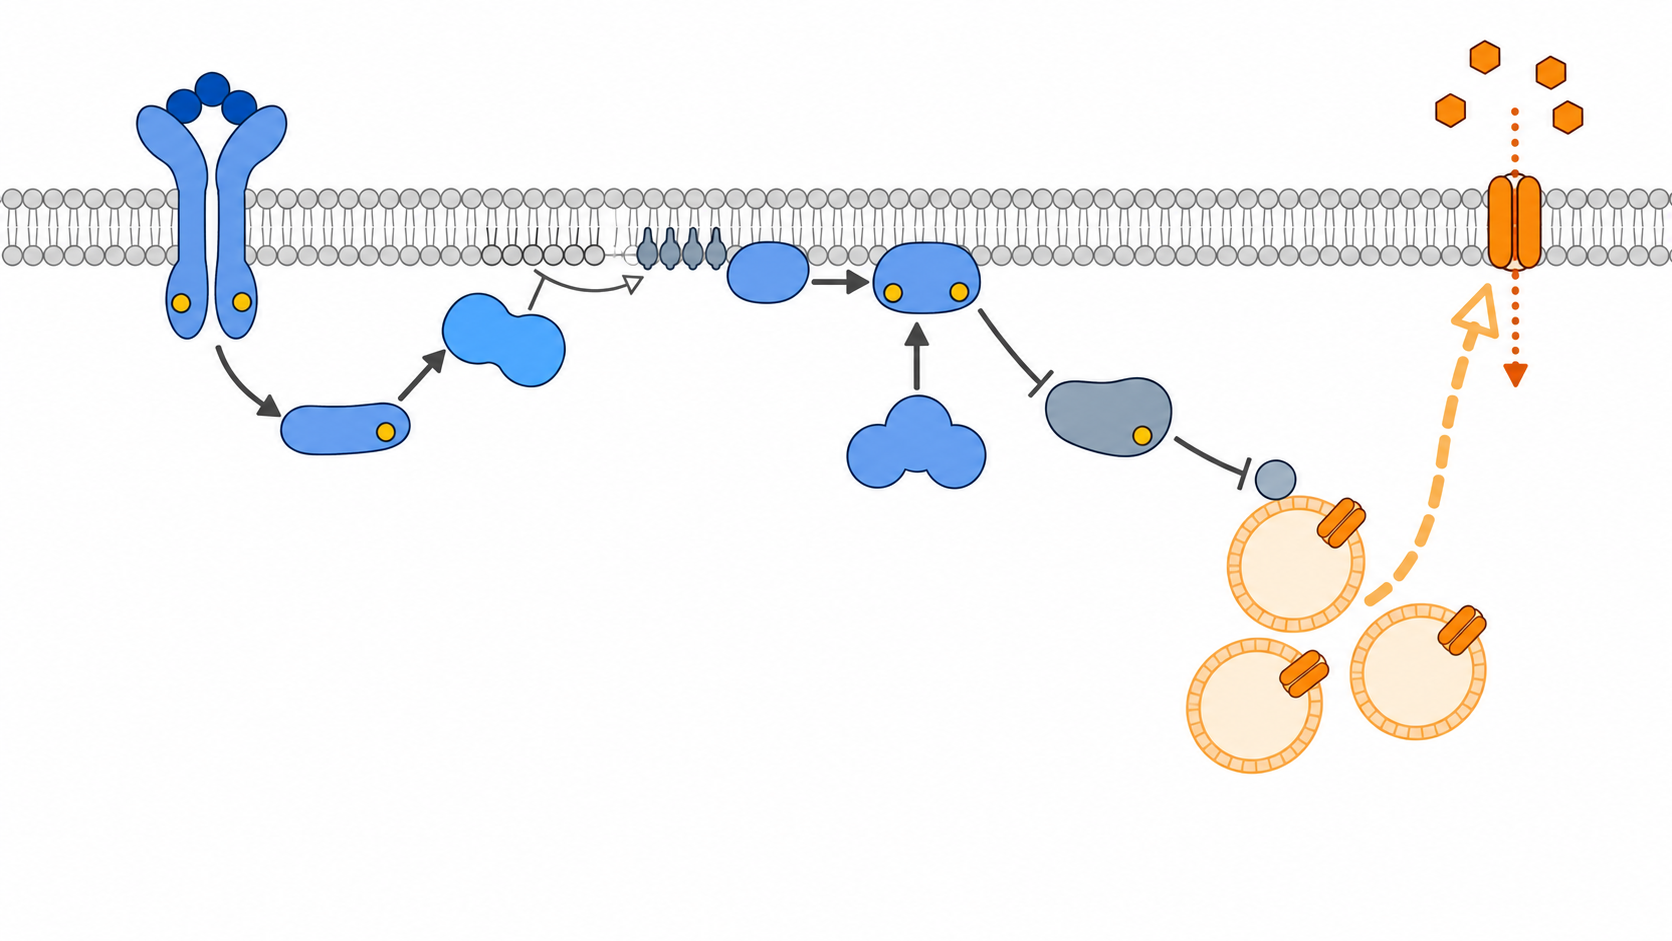
\includegraphics[width=\linewidth]{figures/ch07/ch07-03b-v2-brief.png}
\caption{Comparison of drafts generated from a one-sentence prompt versus a full figure brief. (a) A first draft from a one-sentence prompt; the model bakes rasterized text directly into a dark 3D background, and red numbers mark the scientific and graphical problems discussed in the text. (b) A text-free draft from the full brief: objects and relations can largely be checked one by one, while colour, line weight and spacing are not yet consistent. Example images in this chapter were produced by an image model; prompts and generation logs are available in the book repository.}\label{fig:ch07-03}
\end{figure}

Inspecting Figure~\ref{fig:ch07-03}a shows why surface polish can mislead. Although the model rendered mostly legible English labels rather than garbled pseudo-letters in this run, every word is baked directly into the dark, shaded bitmap. Reduced to a 174 mm double-column print width, small labels over glowing backgrounds become hard to read, and neither font size nor spelling can be edited later. More importantly, checking the image against Table~\ref{tab:ch07-01} exposes seven substantive errors (red circles 1--7 in Figure~\ref{fig:ch07-03}a):
\begin{enumerate}
\item \textbf{Incorrect ligand binding and excessive 3D styling (1):} Extracellular insulin points to the receptor via a white arrow instead of direct contact (violating R1), while heavy highlights, shadows, and glowing ``P'' orbs obscure protein boundaries.
\item \textbf{Multiplicity violation and baked-in prose (2):} Six blue GLUT4 channels crowd a single upper-right membrane pit (violating the single-node rule), alongside three lines of explanatory text about SNAREs baked into the cytosol.
\item \textbf{Inverted causal logic, missing branch, and localization errors (3):} First, \textbf{mTORC2 is completely missing} (omitting R8). Second, \textbf{Akt to AS160 is drawn as a solid white activation arrow} (violating R9), whereas AS160 to Rab uses a red T-bar (R10)---claiming that Akt \emph{activates} AS160 to \emph{inhibit} Rab, the exact opposite of biology! Furthermore, $\text{PIP}_3$ connects via arrows to PDK1 and Akt floating far from the membrane (violating R6), and the green Rab sphere floats free in the cytosol instead of sitting on a vesicle (violating R10).
\item \textbf{Irrelevant organelles filling half the canvas (4):} A huge nucleus, endoplasmic reticulum, and Golgi stack dominate the lower left, crowding the signaling pathway.
\item \textbf{Ambiguous cytoskeleton and looping vesicle arrows (5):} Microtubules and actin filaments fill the lower right while curved arrows connect four cut-away vesicles in a loop, obscuring the storage pool and translocation direction.
\item \textbf{Overlapping upstream nodes and faulty catalysis (6):} IRS-1 and PI3K overlap without a clear activation arrow (obscuring R4), and PI3K points at $\text{PIP}_2$ itself rather than the midpoint of the $\text{PIP}_2 \rightarrow \text{PIP}_3$ conversion arc (violating R5).
\item \textbf{Uniform arrows and missing legend (7):} Apart from one red T-bar, binding, catalysis, activation, vesicle movement, and glucose entry all share the same solid white arrow, with no legend.
\end{enumerate}

Why must both consecutive T-bars be kept in the Akt $\dashv$ AS160 $\dashv$ Rab segment (R9--R10)? In the basal state, AS160 has active Rab-GAP activity that keeps vesicle-associated Rab in its inactive GDP-bound form, acting like a brake that retains vesicles in the cytosol (Sano et al., 2003; Leto and Saltiel, 2012). Akt phosphorylates and \textbf{inhibits} AS160, releasing that brake so Rab remains GTP-bound and promotes vesicle translocation. Collapsing those steps into a single ``Akt $\rightarrow$ GSV'' shortcut arrow erases the mechanism, whereas drawing activation followed by inhibition (Figure~\ref{fig:ch07-03}a) reverses the causal sign.

Now examine Figure~\ref{fig:ch07-03}b, generated from the full brief. When we ran this prompt twice, the first candidate mistakenly routed the T-bar into AS160 from mTORC2 instead of Akt and placed two Rab beads on the vesicles; the second candidate (Figure~\ref{fig:ch07-03}b) fixed both connections. Here the ``extracellular--membrane--cytoplasm'' zones are clear, all thirteen objects and six amber phosphorylation dots are in place, and all five line styles are distinct without extra organelles or baked-in text. Structural accuracy comes from a complete brief paired with line-by-line verification.

\section{One Meaning per Line, One Role per Colour}

During refinement, two visual mistakes frequently creep in: varying arrow styles, weights, and colours arbitrarily, and painting every protein a different saturated hue. Two controlled comparisons illustrate the rules.

The first pair (Figure~\ref{fig:ch07-04}) isolates ``Akt $\dashv$ AS160 $\dashv$ Rab $\rightarrow$ vesicle translocation to membrane GLUT4.'' Figure~\ref{fig:ch07-04}a deliberately mixes four lines: a thick curved red filled arrow from the blue oval to the grey-blue shape (turning inhibition into activation), a thin green dashed open arrow from the grey-blue shape to the vesicle bead, a solid black filled arrow from the vesicles to the membrane transporter identical to a standard activation arrow (implying vesicles ``activate'' GLUT4), and an undefined purple double-headed arrow between the blue oval and the membrane. Figure~\ref{fig:ch07-04}b uses just three lines of two types: two equal-weight dark-grey T-bars in series for double inhibition, and one thick dashed soft-orange open-headed arrow curving upward for spatial translocation (zooming in still shows narrow gaps at the T-bar tips and slight shading on the shapes). Even without text, Figure~\ref{fig:ch07-04}b cleanly separates negative regulation from physical movement.

\begin{figure}[htbp]\centering
\begin{minipage}[t]{0.48\linewidth}\centering
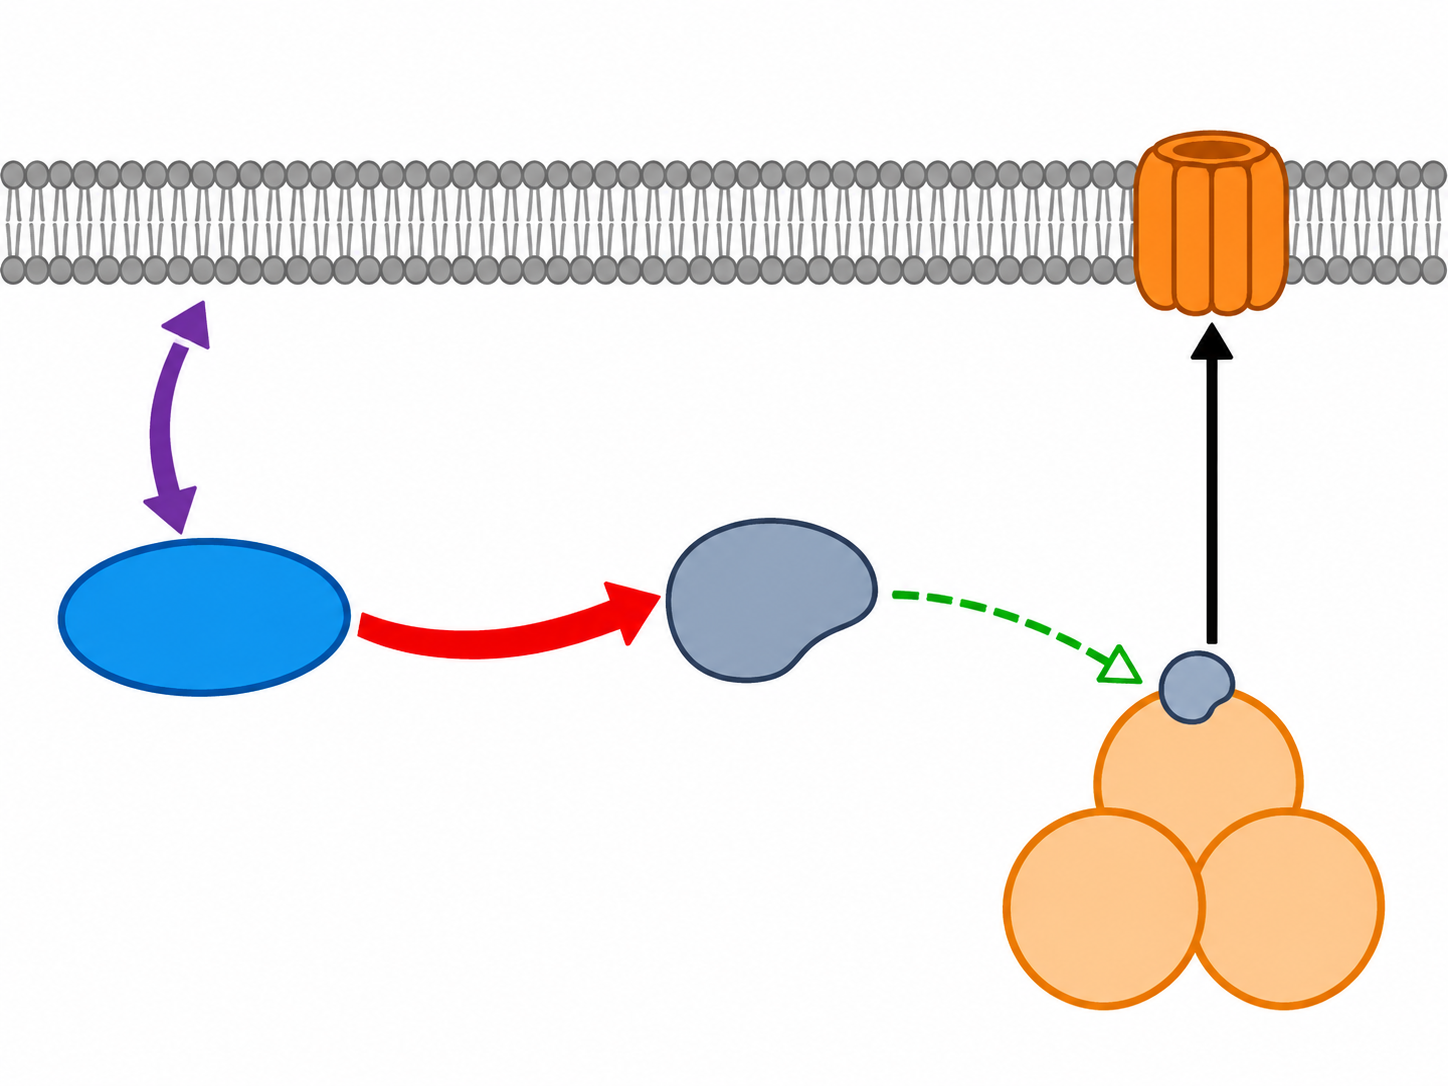
\includegraphics[width=\linewidth]{figures/ch07/ch07-04a-mixed-arrows.png}\\[1mm]
{\footnotesize (a) Mixed line styles: inhibition, translocation, and bidirectional arrows conflated}
\end{minipage}\hfill
\begin{minipage}[t]{0.48\linewidth}\centering
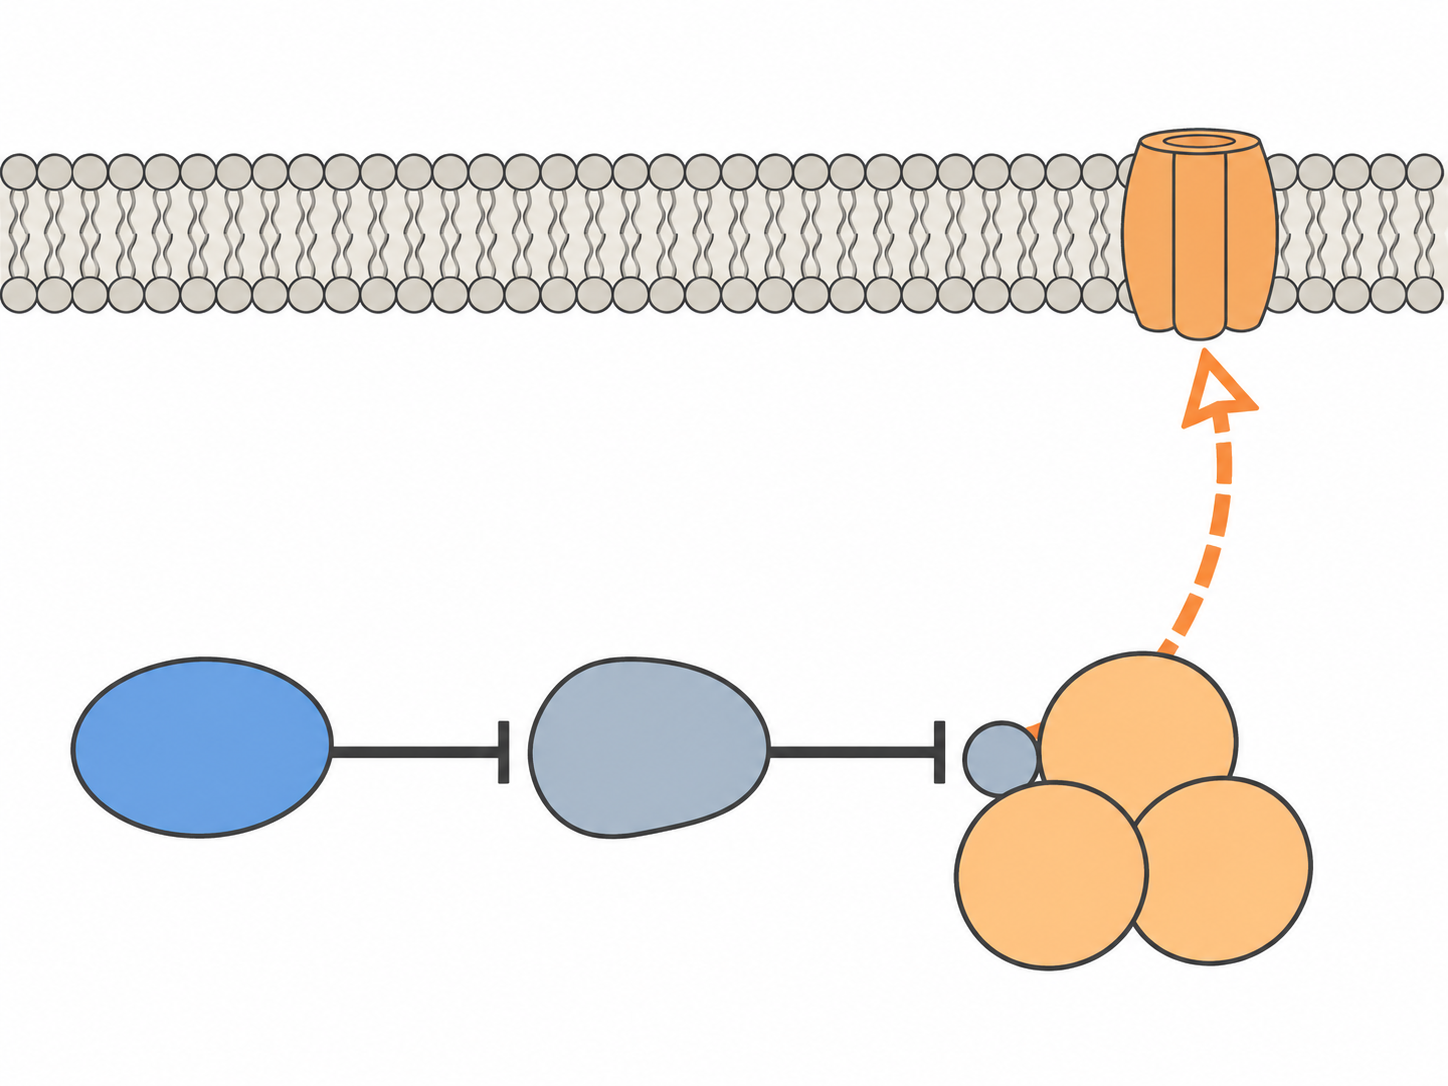
\includegraphics[width=\linewidth]{figures/ch07/ch07-04b-unified-arrows.png}\\[1mm]
{\footnotesize (b) Unified line semantics: two consecutive T-bars and one dashed translocation arrow}
\end{minipage}
\caption{Two drawings of the same simplified pathway. (a) Line style, colour and weight vary at random, the translocation arrow looks like an activation arrow, and a double-headed arrow has no defined meaning. (b) Two T-bars in series read as inhibition of an inhibitor, and the thick dashed arrow is the only symbol for spatial translocation.}\label{fig:ch07-04}
\end{figure}

The second pair (Figure~\ref{fig:ch07-05}) compares an overloaded palette against a restrained role-based palette, together with greyscale conversions.

\begin{figure}[htbp]\centering
\begin{minipage}[t]{0.48\linewidth}\centering
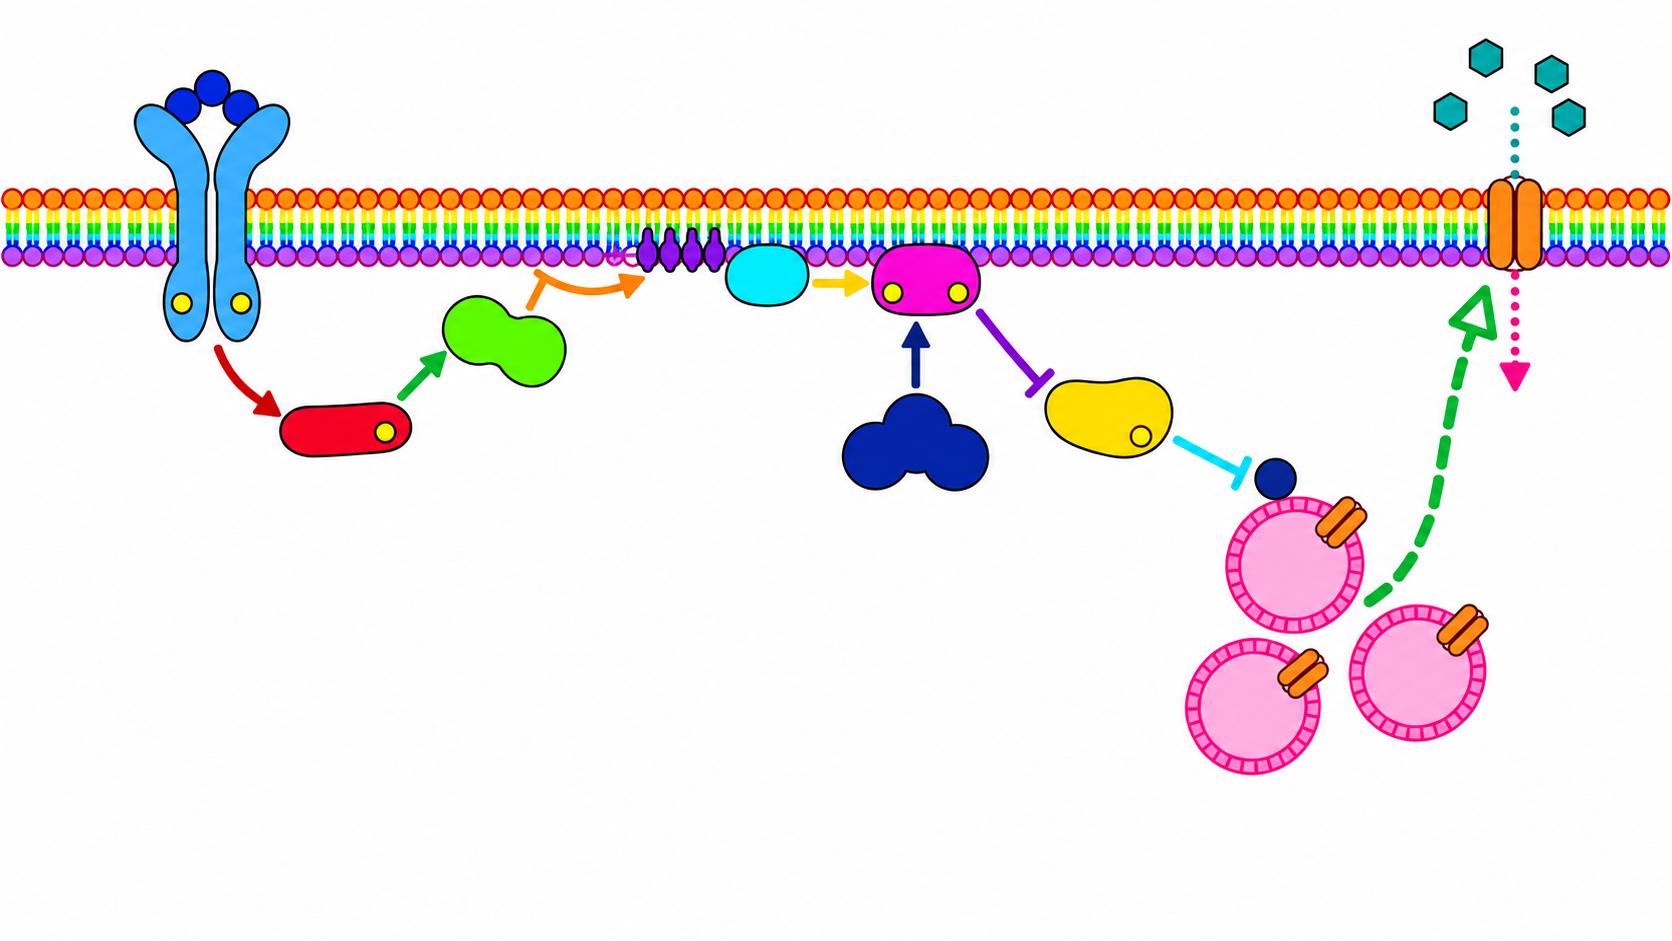
\includegraphics[width=\linewidth]{figures/ch07/ch07-05a-many-colours.png}\\[1mm]
{\footnotesize (a) Unrestrained palette: a different saturated hue per protein and a rainbow membrane}
\end{minipage}\hfill
\begin{minipage}[t]{0.48\linewidth}\centering
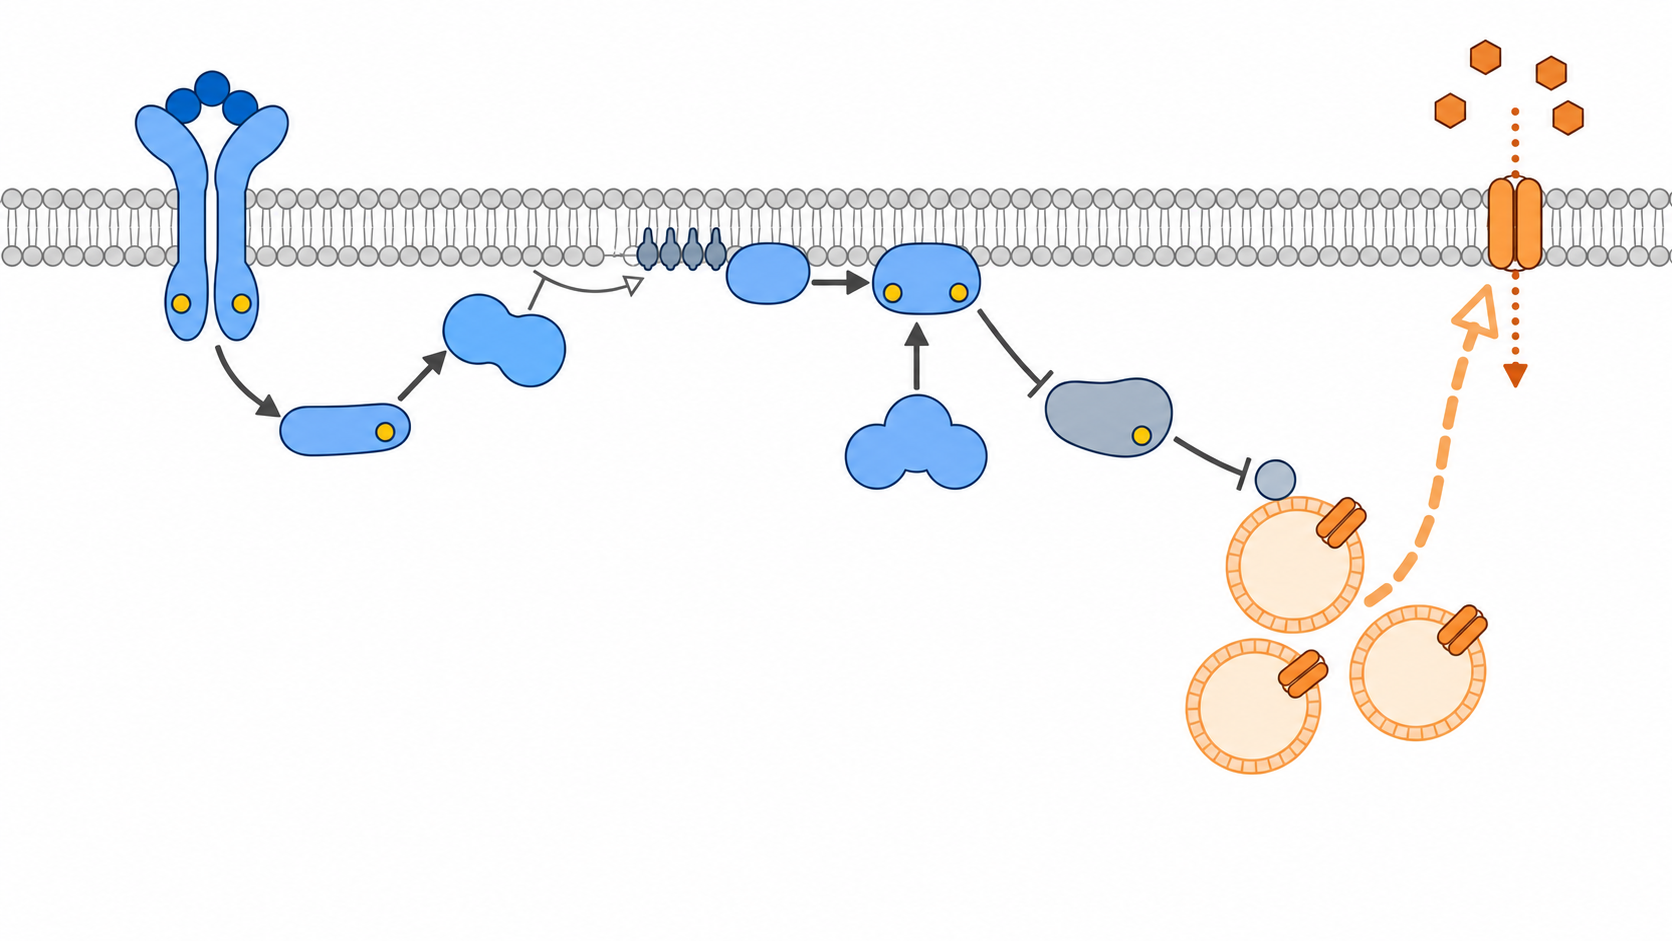
\includegraphics[width=\linewidth]{figures/ch07/ch07-05b-v3-revised.png}\\[1mm]
{\footnotesize (b) Restrained palette (V3): three functional hues plus neutral grey}
\end{minipage}

\vspace{2mm}
\begin{minipage}[t]{0.48\linewidth}\centering
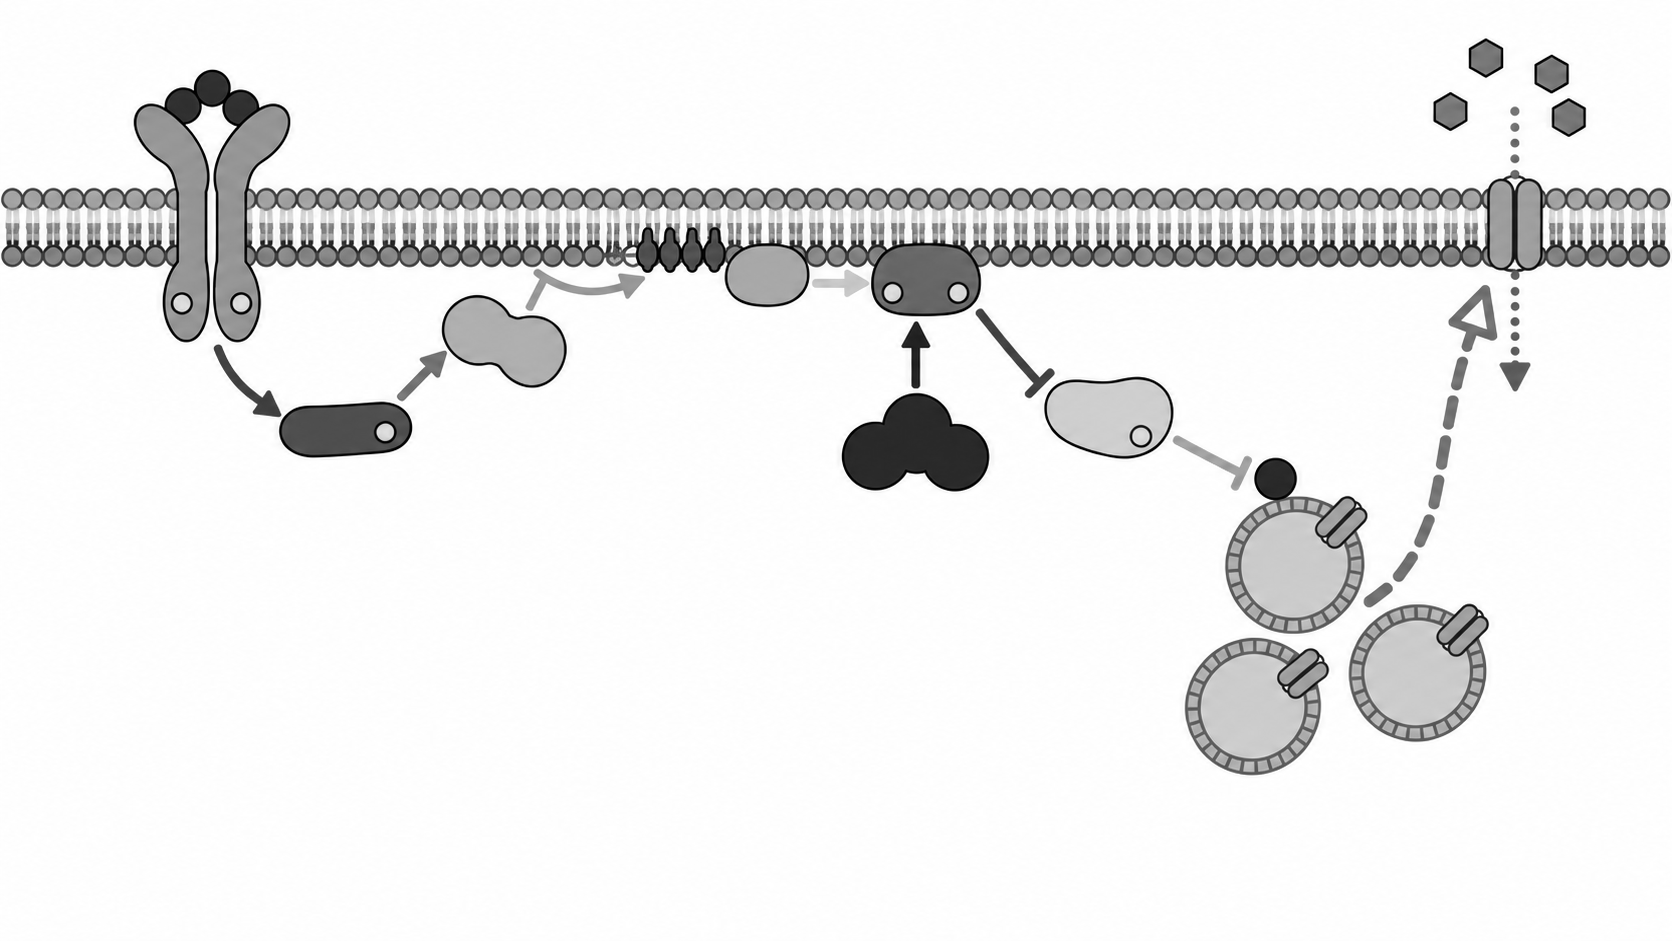
\includegraphics[width=\linewidth]{figures/ch07/ch07-05a-many-colours-gray.png}\\[1mm]
{\footnotesize (c) Greyscale conversion of panel (a)}
\end{minipage}\hfill
\begin{minipage}[t]{0.48\linewidth}\centering
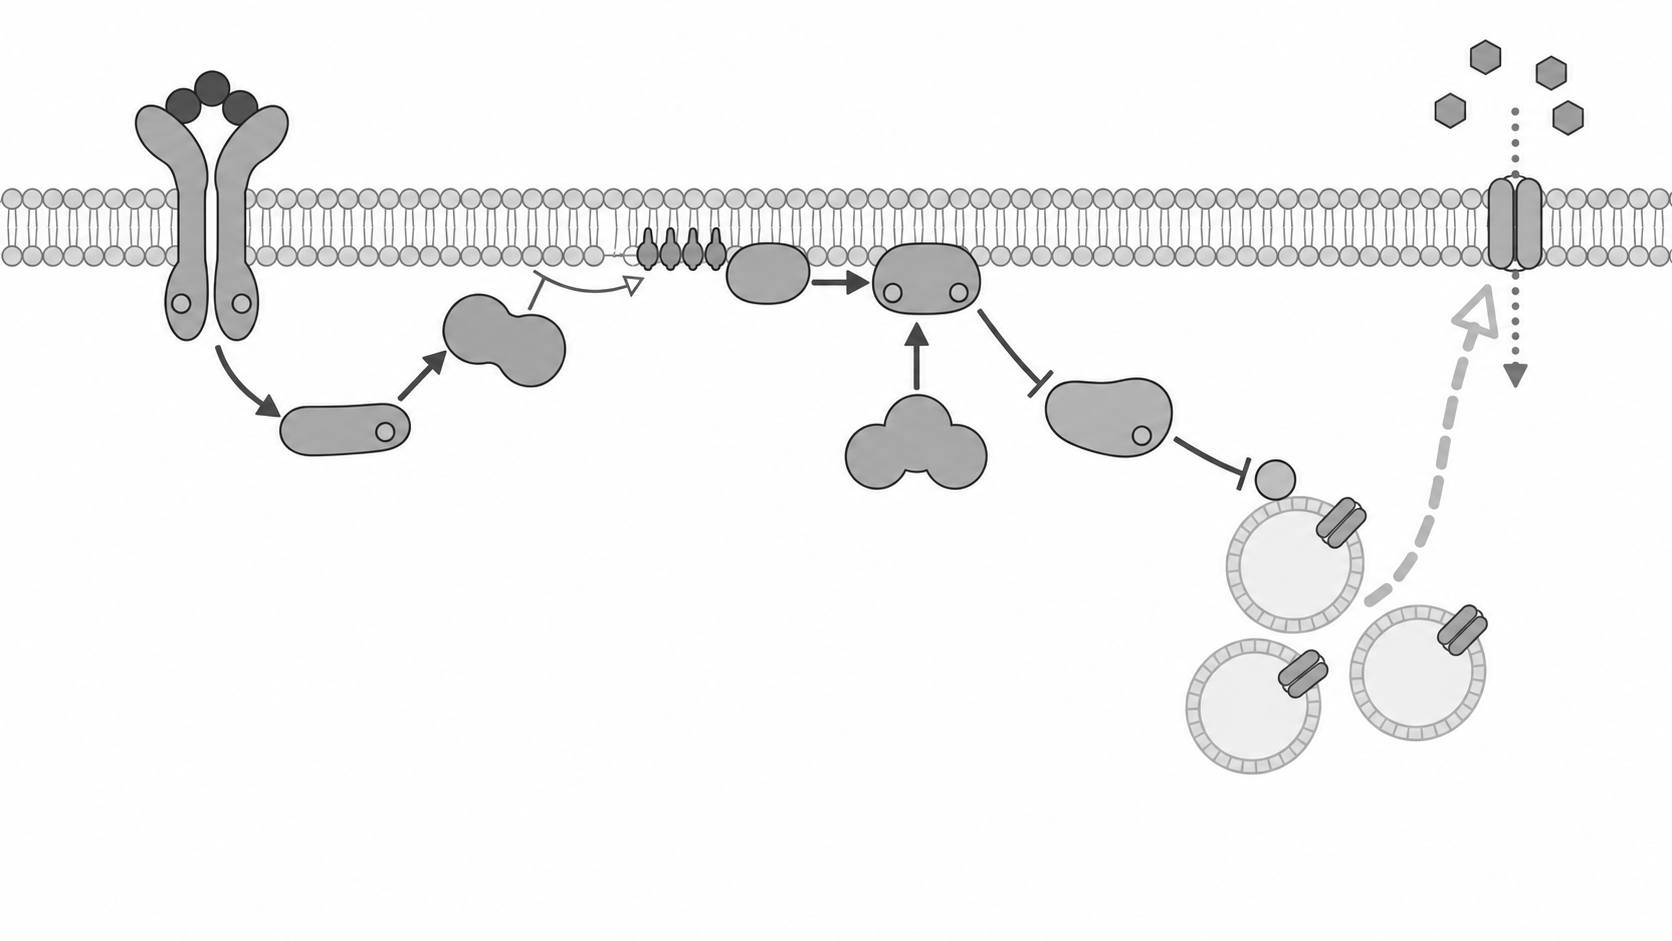
\includegraphics[width=\linewidth]{figures/ch07/ch07-05b-v3-revised-gray.png}\\[1mm]
{\footnotesize (d) Greyscale conversion of panel (b)}
\end{minipage}
\caption{Colour restraint and greyscale testing in mechanism schematics. (a) A different saturated colour for every protein and a rainbow membrane: colour carries no meaning. (b) The revised draft (V3) uses three hues plus grey, one each for signalling proteins, transport regulators, and the transported substance with its carriers. Bottom row: greyscale versions; the hierarchy and line types of (b) remain readable.}\label{fig:ch07-05}
\end{figure}

Generating Figure~\ref{fig:ch07-05}a also underscored model instability: when we first requested a different saturated colour per protein and a rainbow membrane without a reference image, the model rewrote the pathway into a single linear six-protein activation chain, dropping both T-bars and mTORC2 and reversing the glucose arrow! Using Figure~\ref{fig:ch07-05}b as a reference image on the second run preserved the layout, though the $\text{PIP}_2 \rightarrow \text{PIP}_3$ arc arrowhead still switched from hollow to filled.

Comparing Figures~\ref{fig:ch07-05}a and~\ref{fig:ch07-05}b illustrates three principles (Rougier et al., 2014; Wong, 2011): first, colour should encode functional roles rather than individual proteins---Figure~\ref{fig:ch07-05}a scatters red, lime, cyan, magenta, navy, and yellow across proteins without grouping (mTORC2 and Rab share navy despite no link), whereas Figure~\ref{fig:ch07-05}b uses just three hues: medium blue for positive signaling proteins, desaturated grey-blue for negative/trafficking regulators (AS160, Rab), and soft orange for cargo and carriers (glucose, GLUT4, vesicles), plus warm grey for the membrane. Second, avoid pairing red and green (Figure~\ref{fig:ch07-05}a), which is inaccessible to readers with red--green colour-vision deficiency (Wong, 2011; see ColorBrewer 2.0). Third, test in greyscale: in Figure~\ref{fig:ch07-05}c the rainbow membrane turns heavy and protein luminance is chaotic, whereas in Figure~\ref{fig:ch07-05}d functional groups keep uniform luminance and all five line types remain distinct by geometry (while showing that the pale-orange dashed translocation arrow turns light in greyscale, prompting an added text label in the final overlay). You can run \scidraw{}'s Figure Checker (\sdtool{figure-checker}) to flag greyscale and colour-vision risks, remembering that it performs technical checks rather than scientific review.

\section{The Worked Case: From Revision to Final}

We now walk through the closed-loop workflow from the V2 draft (Figure~\ref{fig:ch07-03}b) to the V3 revision (Figure~\ref{fig:ch07-05}b), the V4 final figure (Figure~\ref{fig:ch07-06}), the figure legend, and the verification log.

\subsection{From V2 to V3: Targeted Revision and Catching Unintended Drift}

Checking V2 (Figure~\ref{fig:ch07-03}b) against Table~\ref{tab:ch07-01} confirms correct backbone topology and object counts, but 200\% inspection shows five remaining issues: (1) the $\text{PIP}_2 \rightarrow \text{PIP}_3$ conversion arc (R5) has a closed hollow triangle head rather than an open V, and the PI3K stub meets its left start rather than its midpoint; (2) in membrane recruitment (R6), Akt sits somewhat far from the $\text{PIP}_3$ head groups; (3) narrow white gaps remain at the T-bar ends (R9, R10) and between the translocation arrow tip and membrane GLUT4 (R12); (4) protein fills retain slight shading gradients; and (5) label whitespace is tight in places, while the canvas width corresponds to ~244 ppi at 174 mm print width, below the 300 ppi journal standard.

Our revision instruction from V2 to V3 states what must stay fixed before listing verifiable changes:

\begin{Prompt}
Keep all objects, spatial compartments, and all 13 relations unchanged, and make only
the following modifications:
1. Unify all six signaling proteins (receptor, IRS-1, PI3K, PDK1, Akt, mTORC2) to the
   same flat medium-blue fill and dark-grey outline; unify AS160 and Rab to the same
   desaturated grey-blue fill.
2. Standardize all activation arrows and inhibition lines to a uniform stroke weight,
   with perpendicular T-bar ends touching their target outlines directly.
3. Make the PIP2 -> PIP3 conversion arc thinner in mid-grey with an open V arrowhead,
   and connect the short stub from PI3K to the midpoint of the arc.
4. Keep insulin beads and glucose hexagons at roughly one-third the size of a protein,
   with the three-vesicle GSV cluster clearly visible.
5. Leave at least one protein-width of clear whitespace around every object, keep the
   bottom 12% completely empty, and include no text or symbols anywhere.
\end{Prompt}

Two attempts at generating V3 highlight the danger of \textbf{unintended changes}. First, regenerating from the full V3 prompt without a reference image caused the model to lose all phosphorylation dots, reduce insulin to two beads detached from the receptor, pull PDK1 and Akt off the membrane, invent an unauthorized PI3K $\rightarrow$ PDK1 activation arrow, and draw multiple GLUT4 barrels per vesicle! Second, attaching V2 as a reference image alongside the revision prompt (yielding Figure~\ref{fig:ch07-05}b) preserved all thirteen objects, six phosphorylation dots, membrane contact, and five line styles without extra arrows, though subtle shading, the left-shifted PI3K stub, and tiny T-bar gaps improved only slightly. Thus, \textbf{every revision must be followed by a full-table re-audit, never a spot check of the edited region alone.}

\subsection{V4 Final Artwork: Text-Free Base Image Plus LaTeX/TikZ Overlay}

Why deliver the final figure as a text-free base image plus a LaTeX/TikZ overlay? Image models cannot be trusted to spell molecular names (turning \texttt{Akt} into \texttt{Act} is a factual error), control point sizes, or keep layout fixed across edits. Placing typography in TikZ lets us copy names directly from the verified table, fix print font sizes at 7--8 pt, and share one raster base across English and Chinese editions by swapping only the overlay file. Delivery can follow \textbf{Option A} (base image includes objects and arrows, TikZ adds labels and legend; used here) or \textbf{Option B} (base image has only objects/layers, TikZ draws both arrows and labels; used in the battery case next).

Using V3 as a reference for the V4 base image, the prompt locked the hex palette and reserved empty label rectangles (full prompt in \texttt{cases/}):

\begin{Prompt}
Final base artwork for a journal Figure 1, flat 2D vector-style scientific
schematic, landscape 16:9, print resolution 300 ppi at 174 mm width, pure white
background, uniform thin dark gray (#3A3A3A) outlines, flat fills, no gradients.
THIS IMAGE MUST CONTAIN NO TEXT AT ALL: no letters, words, numbers, or "P".
PALETTE: signaling proteins #A9C4E0 / #4C78A8; insulin #2F5D8C; AS160 and Rab
#B8C2CC; GLUT4 and vesicles #F2C49B / #E39B5B; glucose #C46A2A; membrane
#D9D6D0 / #BDB8AF; phosphorylation dots #E3B23C; lines #3A3A3A and #7A7A7A.
LAYOUT & RELATIONS: keep the same 13 objects, phosphorylation dots, and 5 line
types as the reference image. Leave generous empty white margins above the
membrane, around each protein, and across the bottom 12% strip for overlaid
labels and the figure legend.
\end{Prompt}

Generating V4 again required catching drift and adjusting in layout: an unreferenced first run drew the vesicle GLUT4 barrels inside the vesicle lumens; conditioning on V3 restored proper membrane embedding, and 200\% inspection of the third run confirmed zero stray text or watermarks. Because object edges still intruded into several reserved label boxes, the PI3K stub still joined the left end of the conversion arc, tiny gaps remained at the T-bars, and resolution stayed at ~244 ppi at 174 mm width, we used a normalized $(0,0)$--$(1,1)$ TikZ coordinate system over the base image to fine-tune the seventeen label positions with short leader lines and typeset a vector legend along the bottom band (Figure~\ref{fig:ch07-06}).

\begin{figure}[htbp]\centering
% FIG ch07-06 GLUT4 final overlay (English)
\definecolor{ch07comp}{HTML}{6B6B6B}
\definecolor{ch07transnote}{HTML}{C46A2A}
\definecolor{ch07act}{HTML}{3A3A3A}
\definecolor{ch07conv}{HTML}{7A7A7A}
\definecolor{ch07trans}{HTML}{E39B5B}
\definecolor{ch07flux}{HTML}{C46A2A}
\definecolor{ch07phos}{HTML}{E3B23C}
\begin{tikzpicture}
  \node[anchor=south west, inner sep=0] (img) at (0,0)
    {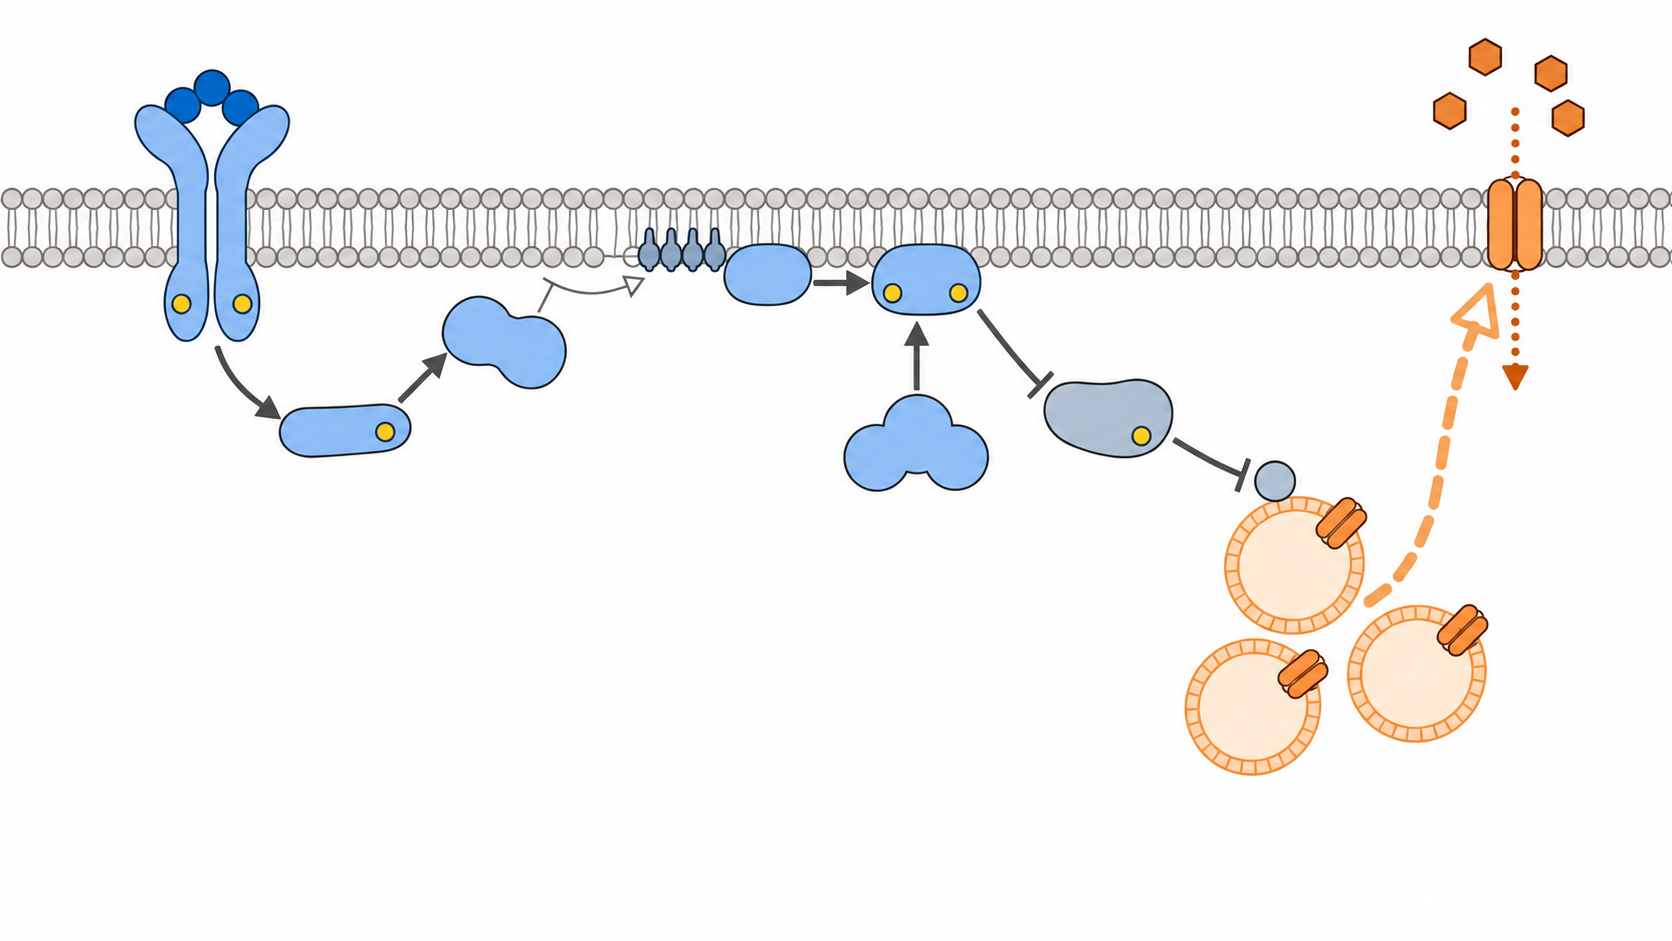
\includegraphics[width=\linewidth]{figures/ch07/ch07-06-v4-base.png}};
  \begin{scope}[x={(img.south east)}, y={(img.north west)},
    font=\sffamily\small]
    \node[text=ch07comp, font=\sffamily\footnotesize\itshape, anchor=west]
      at (0.04, 1-0.055) {Extracellular};
    \node[text=ch07comp, font=\sffamily\footnotesize\itshape]
      at (0.62, 1-0.15) {Plasma membrane};
    \node[text=ch07comp, font=\sffamily\footnotesize\itshape, anchor=west]
      at (0.04, 1-0.90) {Cytoplasm};
    \node[anchor=west, font=\sffamily\small] at (0.20, 1-0.06) {Insulin};
    \draw[BookInk!40, thin] (0.20, 1-0.065) -- (0.145, 1-0.10);
    \node[anchor=west, font=\sffamily\small] at (0.20, 1-0.145) {Insulin receptor};
    \draw[BookInk!40, thin] (0.20, 1-0.15) -- (0.16, 1-0.20);
    \node[font=\sffamily\small] at (0.21, 1-0.56) {IRS-1};
    \node[font=\sffamily\small] at (0.34, 1-0.50) {PI3K};
    \node[font=\sffamily\footnotesize] at (0.48, 1-0.075) {PIP\textsubscript{2} → PIP\textsubscript{3}};
    \draw[BookInk!40, thin] (0.44, 1-0.10) -- (0.385, 1-0.275);
    \node[font=\sffamily\small] at (0.46, 1-0.40) {PDK1};
    \node[font=\sffamily\small] at (0.515, 1-0.375) {Akt};
    \draw[BookInk!40, thin] (0.53, 1-0.36) -- (0.55, 1-0.335);
    \node[font=\sffamily\small] at (0.52, 1-0.60) {mTORC2};
    \draw[BookInk!40, thin] (0.54, 1-0.56) -- (0.55, 1-0.52);
    \node[align=center, font=\sffamily\footnotesize] at (0.80, 1-0.345) {AS160\\(TBC1D4)};
    \draw[BookInk!40, thin] (0.755, 1-0.385) -- (0.695, 1-0.42);
    % Two short lines in the white gap right of the Rab circle (x 0.78–0.84).
    \node[align=left, font=\sffamily\scriptsize, anchor=south west] at (0.788, 1-0.508) {Rab-\\GTP};
    \draw[BookInk!40, thin] (0.784, 1-0.500) -- (0.770, 1-0.512);
    \node[align=center, font=\sffamily\small, anchor=north] at (0.78, 1-0.85) {GLUT4 storage\\vesicles};
    \draw[BookInk!40, thin] (0.78, 1-0.845) -- (0.78, 1-0.80);
    \node[font=\sffamily\small, anchor=west] at (0.94, 1-0.345) {GLUT4};
    \draw[BookInk!40, thin] (0.94, 1-0.33) -- (0.915, 1-0.26);
    \node[font=\sffamily\small, anchor=east] at (0.845, 1-0.065) {Glucose};
    \draw[BookInk!40, thin] (0.845, 1-0.075) -- (0.875, 1-0.09);
    % Right-aligned beside the dashed arrow; the long line stays right of x=0.87.
    \node[text=ch07transnote, font=\sffamily\scriptsize\itshape, align=right, anchor=north east]
      at (0.998, 1-0.430) {translocation\\\& fusion};
    \draw[ch07transnote!55, thin] (0.878, 1-0.448) -- (0.858, 1-0.432);
  \end{scope}
  \node[anchor=north west, font=\sffamily\scriptsize, align=left] at (img.south west) {%
    \begin{tabular}{@{}l@{\quad}l@{}}
      \tikz{\draw[-{Stealth[length=1.5mm]}, ch07act, line width=0.6pt] (0,0) -- (0.22,0);} Activation &
      \tikz{\draw[-{Bar[width=4pt]}, ch07act, line width=0.6pt] (0,0) -- (0.22,0);} Inhibition \\
      \tikz{\draw[ch07conv, line width=0.4pt] (0,0) .. controls (0.08,0.04) .. (0.18,0);} Enz.\ conv. &
      \tikz{\draw[ch07trans, line width=1pt, dashed] (0,0) -- (0.18,0);} Translocation \\
      \tikz{\draw[ch07flux, line width=0.6pt, dotted, -{Stealth[length=1.2mm]}] (0,0) -- (0.18,0);} Glucose flux &
      \tikz{\fill[ch07phos] (0.09,0) circle (1.2pt);} Phosphorylation
    \end{tabular}};
\end{tikzpicture}

\caption{Final schematic of the canonical insulin pathway leading to GLUT4 translocation. The text-free base image was generated by an image model; labels and legend are typeset in LaTeX on top. Solid lines with filled heads, activation; T-bars, inhibition; thin arc, enzymatic conversion; thick dashed arrow, vesicle translocation; dotted arrow, glucose flux; amber dots, phosphorylation. The MAPK and CAP--Cbl--TC10 branches, GLUT4 endocytosis and recycling, negative feedback, SNARE fusion machinery and cytoskeletal transport are omitted; Akt and Rab isoforms are not distinguished, and upstream regulation of mTORC2 is not shown. Based on Saltiel and Kahn (2001), Leto and Saltiel (2012) and Klip et al.\ (2019). The full caption is given in the text.}\label{fig:ch07-06}
\end{figure}

\subsection{Full Figure Legend, Self-Check, and Verification Log}

If you draft a caption with \scidraw{}'s Figure Legend assistant (\sdtool{figure-legend}), use it only as a rough outline and never let it fabricate sample sizes or statistical tests. The complete caption reads:

\begin{BookNote}
\textbf{Figure 1 | Schematic of the canonical insulin signaling pathway leading to GLUT4 translocation.} Insulin binding to the insulin receptor at the plasma membrane triggers tyrosine autophosphorylation of the receptor's intracellular domain, which phosphorylates IRS-1 and recruits class IA PI3K. PI3K converts $\text{PIP}_2$ to $\text{PIP}_3$ in the inner leaflet; $\text{PIP}_3$ recruits PDK1 and Akt, and Akt is activated by phosphorylation by PDK1 and mTORC2. Active Akt phosphorylates AS160 (TBC1D4), inhibiting its Rab-GAP activity. Rab proteins on GLUT4 storage vesicles therefore remain GTP-bound, promoting vesicle translocation to and fusion with the plasma membrane. The resulting increase in surface GLUT4 allows facilitated diffusion of glucose into the cell. Solid lines with filled heads, activation; T-bars, inhibition; thin arc, enzymatic conversion; thick dashed arrow, vesicle translocation; dotted arrow, glucose flux; amber dots, phosphorylation. For clarity, the MAPK and CAP--Cbl--TC10 branches, GLUT4 endocytosis and recycling, negative feedback, the SNARE fusion machinery and cytoskeletal transport are omitted; Rab and Akt isoforms are not distinguished, the parallel role of TBC1D1 in skeletal muscle is not shown, and upstream regulation of mTORC2 is not depicted. Based on reviews by Saltiel and Kahn (2001), Leto and Saltiel (2012) and Klip et al.\ (2019).
\end{BookNote}

A sentence-by-sentence check confirms that the opening sentences map sequentially to R1--R4, R5--R8, and R9--R13; the next sentence defines all six legend symbols; the following sentence states all omissions; and the final sentence cites the literature, with no data or statistical terms. Table~\ref{tab:ch07-verify} excerpts the V4 verification log, separating the author verifier from the domain peer reviewer---neither AI nor technical checks can replace peer review.

\begin{table}[htbp]\centering\scriptsize
\setlength{\tabcolsep}{3pt}
\renewcommand{\arraystretch}{1.1}
\caption{Excerpt from the verification log for the GLUT4 V4 base artwork. Author verifier: first author; domain peer reviewer: metabolism co-author (pending sign-off).}\label{tab:ch07-verify}
\begin{tabularx}{\linewidth}{lYYYY}
\toprule
\textbf{Audit item} & \textbf{Brief specification} & \textbf{Observed V4 result} & \textbf{Status} & \textbf{Disposition} \\
\midrule
R1--R4, R7--R8, R13 & Ligand contact, phosphorylation dots, 4 activation lines, no mTORC2 upstream line, dotted membrane flux & Counts, directions, amber dots, and line styles match brief & Pass & Keep and overlay TikZ labels \\
R5 enzymatic conversion & $\text{PIP}_2 \rightarrow \text{PIP}_3$ thin arc, open V head, PI3K stub at midpoint & Arc points right, but head is closed hollow triangle and stub joins left end & Partial deviation & Logged for teaching draft; redraw in TikZ for submission \\
R6 membrane recruitment & PDK1, Akt touch inner leaflet at $\text{PIP}_3$, no arrow & Both touch inner leaflet without arrows; Akt slightly far from $\text{PIP}_3$ & Partial deviation & Place label between PI3K and PDK1 to aid reading \\
R9--R10 double inhibition & Akt $\dashv$ AS160 $\dashv$ Rab perpendicular T-bars touching targets & Series T-bars correct, Rab on upper-left vesicle; narrow gap at T-bar tips & Partial deviation & Meaning clear; use Option B if strict contact needed \\
R11--R12 translocation & Thick dashed orange arrow to membrane GLUT4; vesicle GLUT4 in membrane & 3 vesicles each embed 1 GLUT4; small gap at dashed arrow tip & Partial deviation & Add ``translocation \& fusion'' label beside arrow \\
No-text \& resolution & No text at 200\% zoom; 300 ppi at 174 mm width & No text at 200\% zoom; ~244 ppi at 174 mm width & Needs higher ppi & Flag as candidate base; do not upscale to fake ppi \\
Unintended changes & Log unrequested edits across rounds & Unreferenced V3 lost dots and added arrow; unreferenced V4 put GLUT4 in lumen & Intercepted & Restored by using prior verified image as reference \\
\bottomrule
\end{tabularx}
\end{table}

\section{Structure Schematics: Layer Order, Materials, and Direction}

For device and materials schematics (battery cells, photovoltaic stacks, membrane assemblies), verification shifts from logical links to four physical dimensions: \textbf{layer sequence} (which layer touches which), \textbf{material pairing} (which collector pairs with which electrode), \textbf{process direction} (paths of ions and electrons), and \textbf{operating state} (charging vs.\ discharging).

Suppose a master's student studying cathode materials wants a pouch-cell cross-section for her thesis introduction. Submitting a single sentence---\texttt{Draw a lithium-ion battery cross-section showing how it charges}---typically yields scrambled layers or reversed ion arrows. Following electrochemical consensus (Goodenough and Park, 2013; Tarascon and Armand, 2001; Armand and Tarascon, 2008; Xu, 2004; Arora and Zhang, 2004; Nitta et al., 2015), we first define the checklist S1--S8 in Table~\ref{tab:ch07-03}.

\begin{table}[htbp]\centering\scriptsize
\setlength{\tabcolsep}{3pt}
\renewcommand{\arraystretch}{1.1}
\caption{Layer-order and process verification table (S1--S8) for a lithium-ion pouch-cell unit cross-section.}\label{tab:ch07-03}
\begin{tabularx}{\linewidth}{lYYYY}
\toprule
\textbf{ID} & \textbf{Item} & \textbf{Correct specification} & \textbf{Common error} & \textbf{Basis} \\
\midrule
S1 & Layer order (left to right) & Pouch film $\rightarrow$ Cu collector $\rightarrow$ negative (graphite) $\rightarrow$ separator $\rightarrow$ positive (e.g.\ $\text{LiCoO}_2$) $\rightarrow$ Al collector $\rightarrow$ pouch film & Separator placed between electrode and collector; electrodes touch directly & Goodenough and Park, 2013; Arora and Zhang, 2004 \\
S2 & Collector pairing & Negative uses Cu foil; positive uses Al foil & Cu and Al swapped & Nitta et al., 2015; textbook convention \\
S3 & Electrolyte location & Wets pores of both electrodes and separator & Drawn as a separate standalone liquid layer & Xu, 2004 \\
S4 & $\text{Li}^+$ during charging & De-intercalates from positive, crosses separator, intercalates into graphite negative (right $\rightarrow$ left) & Direction reversed (left $\rightarrow$ right) & Goodenough and Park, 2013 \\
S5 & Electrons during charging & Positive $\rightarrow$ external circuit (charger) $\rightarrow$ negative & Electrons cross separator/electrolyte & Same as above \\
S6 & Discharging $\text{Li}^+$ / $\text{e}^-$ & $\text{Li}^+$ negative $\rightarrow$ positive (left $\rightarrow$ right) in electrolyte; $\text{e}^-$ negative $\rightarrow$ load $\rightarrow$ positive & Directions not reversed with state & Same as above \\
S7 & $\text{Li}^+$ path & Migrates only inside cell (in electrolyte) & $\text{Li}^+$ drawn in external wire & Same as above \\
S8 & Nomenclature & Label ``Negative / Positive electrode''; note in caption that anode/cathode follow discharge convention & Labelling anode/cathode on charging plot without note, or swapping them & Textbook convention \\
\bottomrule
\end{tabularx}
\end{table}

We first generated Figure~\ref{fig:ch07-07} from a deliberately error-inducing prompt so readers can spot four common mistakes against Table~\ref{tab:ch07-03}: (1) the left graphite negative electrode is paired with silver-grey Al foil and the right positive electrode with Cu foil (swapped collectors, violating S2); (2) graphite flakes and slate-blue positive oxide particles touch directly (an internal short circuit in a real cell) while the white porous separator sits between the positive electrode and the right Cu foil (violating S1); (3) the panel is labelled ``Charging,'' yet all six orange $\text{Li}^+$ spheres inside the electrodes point right, from negative to positive (violating S4); and (4) three orange $\text{Li}^+$ spheres with arrows travel along the top external wire (violating S7).

\begin{figure}[htbp]\centering
% FIG ch07-07 battery common errors overlay (English)
\definecolor{ch07err}{HTML}{C0392B}
\begin{tikzpicture}
  \node[anchor=south west, inner sep=0] (img) at (0,0)
    {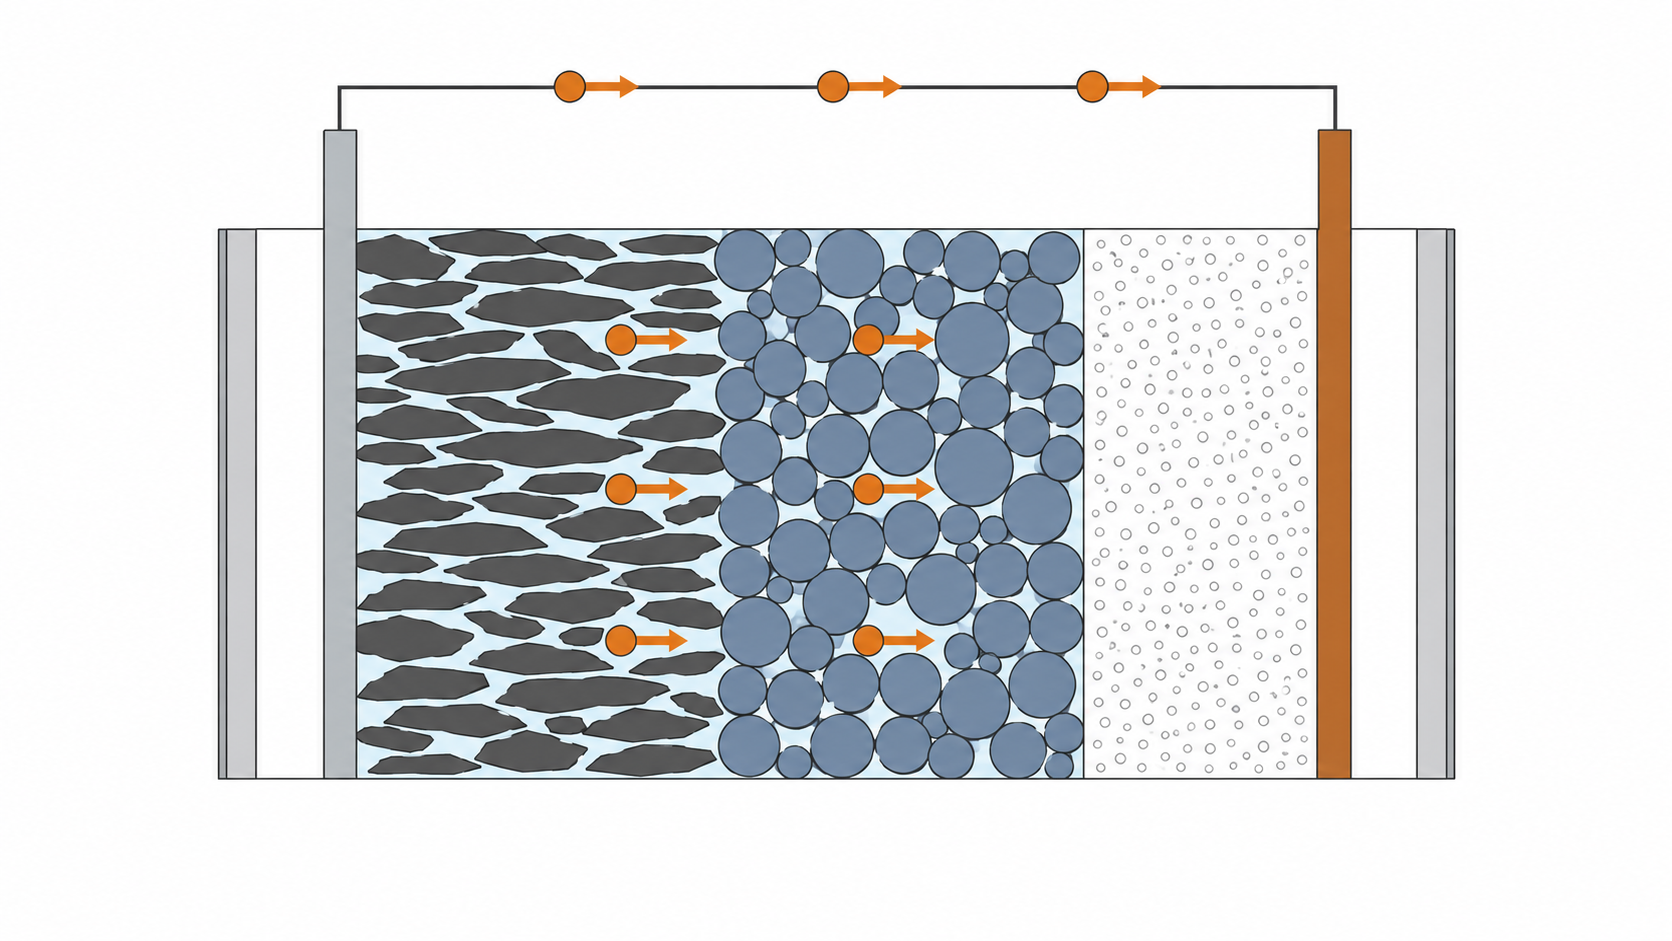
\includegraphics[width=\linewidth]{figures/ch07/ch07-07-battery-errors.png}};
  \begin{scope}[x={(img.south east)}, y={(img.north west)},
    font=\sffamily\small]
    \node[font=\bfseries] at (0.50, 1-0.02) {Charging (incorrect example)};
    \node[font=\scriptsize] at (0.20, 1-0.90) {Al foil};
    \node[font=\scriptsize, align=center] at (0.315, 1-0.90) {Negative\\(graphite)};
    \node[font=\scriptsize, align=center] at (0.525, 1-0.90) {Positive\\(e.g.\ LiCoO$_2$)};
    \node[font=\scriptsize] at (0.69, 1-0.90) {Separator};
    \node[font=\scriptsize] at (0.76, 1-0.94) {Cu foil};
    \node[font=\scriptsize, rotate=90, anchor=south] at (0.15, 1-0.20) {Pouch};
    \node[font=\scriptsize] at (0.20, 1-0.11) {Negative tab};
    \node[font=\scriptsize] at (0.76, 1-0.11) {Positive tab};
    \node[font=\scriptsize\bfseries, text=white, fill=ch07err, circle, inner sep=1.5pt] at (0.20, 1-0.22) {1};
    \node[font=\scriptsize\bfseries, text=white, fill=ch07err, circle, inner sep=1.5pt] at (0.76, 1-0.22) {1};
    \node[font=\scriptsize\bfseries, text=white, fill=ch07err, circle, inner sep=1.5pt] at (0.42, 1-0.22) {2};
    \node[font=\scriptsize\bfseries, text=white, fill=ch07err, circle, inner sep=1.5pt] at (0.40, 1-0.55) {3};
    \node[font=\scriptsize\bfseries, text=white, fill=ch07err, circle, inner sep=1.5pt] at (0.50, 1-0.08) {4};
    \node[font=\scriptsize, text=BookInk!80, anchor=north] at (0.50, 1-0.96)
      {1--4 map to checklist S2, S1, S4, S7 in Table~7-3};
  \end{scope}
\end{tikzpicture}

\caption{A deliberately incorrect battery schematic, generated by an image model from a prompt that specified the errors. (1) The copper and aluminium current collectors are swapped. (2) The separator is not between the electrodes, so the electrodes touch, which in a real cell means an internal short circuit. (3) The panel is labelled as charging, yet Li$^+$ moves from the negative to the positive electrode. (4) Li$^+$ is drawn travelling through the external circuit. See Figure~\ref{fig:ch07-08} for the correct version.}\label{fig:ch07-07}
\end{figure}

Why does the correct figure (Figure~\ref{fig:ch07-08}) exclude arrows from the AI base image? Because arrow direction is the core scientific content and reverses between charging and discharging; generating two separate images would cause random drift in layer widths and particle packing, implying that the cell structure changes between states. We therefore generate the structure-only base image once and overlay both sets of process arrows in TikZ:

\begin{Prompt}
[Purpose & Audience] Introductory structure schematic (double-column width 174 mm, two
panels side by side) for materials science and electrochemistry readers.
[Goal] Show the exact layer sequence and collector pairing of a single repeating unit of
a lithium-ion pouch cell, and contrast the internal Li+ and external electron paths
between charging and discharging.
[Objects & Counts] Each structural layer appears once from left to right: outer pouch
film, copper current collector with top tab, graphite negative electrode coating,
porous separator, layered-oxide positive electrode coating (e.g., LiCoO2), aluminium
current collector with top tab, outer pouch film; pale-blue electrolyte filling pores.
[Process Overlay (in TikZ only, absent from base image)]
(a) Charging: Li+ from positive -> separator -> negative; e- from positive tab -> charger -> negative tab.
(b) Discharging: Li+ from negative -> separator -> positive; e- from negative tab -> load -> positive tab.
Li+ stays strictly inside the electrolyte; electrons stay strictly in the external wire.
[Layout & Visuals] 16:9 cross-section; vertical layer bands across x 0.14-0.86; top and
bottom margins empty for external circuit and legend. Flat 2D vector style on white.
[Restrictions] Base image contains NO text, symbols, +/- signs, ions, electrons, arrows,
or wires; omit SEI layer, binder, conductive carbon, and packaging seals; not to scale.
\end{Prompt}

Across three runs of this base prompt, the first run added two unwanted pale-blue vertical bands between the pouch films and collectors that looked like standalone liquid layers (violating S3), and the third left the separator pores white with sparse positive particles. The second run cleanly produced the sequence ``pouch film--Cu collector--flaky graphite negative--central porous separator--spherical oxide positive--Al collector--pouch film'' with no ions, wires, or text (zooming in shows only slight unevenness in the pale-blue separator pores). In LaTeX, we called this single base image twice side by side and overlaid the top external circuit (charger or load), dashed electron arrows ($\text{e}^-$), and solid orange internal $\text{Li}^+$ arrows in TikZ (Figure~\ref{fig:ch07-08}). Note that converting a bitmap to PPTX or SVG only separates text from background rather than turning particles or separators into semantically editable objects, so directional arrows belong in TikZ or vector software.

\begin{figure}[htbp]\centering
% FIG ch07-08 charge/discharge overlay (English)
\definecolor{ch07Li}{HTML}{D9822B}
\definecolor{ch07wire}{HTML}{3A3A3A}
\definecolor{ch07elec}{HTML}{3A3A3A}
\definecolor{ch07electrolyte}{HTML}{E3F0F8}
\begin{tikzpicture}
  \node[anchor=south west, inner sep=0] (imgA) at (0,0)
    {\includegraphics[width=0.49\linewidth]{\chsevenpanelbase}};
  \node[anchor=south west, inner sep=0] (imgB) at (0.51\linewidth,0)
    {\includegraphics[width=0.49\linewidth]{\chsevenpanelbase}};
  \begin{scope}[shift={(imgA.south west)},
    x={($(imgA.south east)-(imgA.south west)$)},
    y={($(imgA.north west)-(imgA.south west)$)},
    font=\sffamily\small]
    \node[anchor=south west, font=\sffamily\small] at (0.00, 1.20) {\textbf{(a)} Charging};
    \node[align=center, font=\sffamily\scriptsize, anchor=north west] at (0.25, 1.045) {Negative\\tab};
    \node[align=center, font=\sffamily\scriptsize, anchor=north east] at (0.75, 1.045) {Positive\\tab};
    \chsevendrawcircuit{Charger}
  \end{scope}
  \begin{scope}[shift={(imgB.south west)},
    x={($(imgB.south east)-(imgB.south west)$)},
    y={($(imgB.north west)-(imgB.south west)$)},
    font=\sffamily\small]
    \node[anchor=south west, font=\sffamily\small] at (0.00, 1.20) {\textbf{(b)} Discharging};
    \chsevendrawcircuitb{Load}
  \end{scope}
  \begin{scope}[shift={(imgA.south west)},
    x={($(imgA.south east)-(imgA.south west)$)},
    y={($(imgA.north west)-(imgA.south west)$)},
    font=\sffamily\scriptsize]
    \node[align=center, anchor=north] at (0.323, 0.19) {Negative\\(graphite)};
    \node[anchor=north] at (0.50, 0.19) {Separator};
    \node[align=center, anchor=north] at (0.678, 0.19) {Positive\\(LiCoO\textsubscript{2})};
    \draw[BookInk!45, thin] (0.193, 0.19) -- (0.193, -0.02);
    \node[align=center, anchor=north] at (0.193, -0.02) {Cu\\collector};
    \draw[BookInk!45, thin] (0.806, 0.19) -- (0.806, -0.02);
    \node[align=center, anchor=north] at (0.806, -0.02) {Al\\collector};
  \end{scope}
  \node[anchor=north, font=\sffamily\scriptsize, align=center] at (0.5\linewidth, -0.13\linewidth) {%
    \begin{tabular}{@{}c@{\qquad}c@{}}
      \tikz{\draw[-{Stealth[length=1.5mm]}, ch07Li, line width=0.7pt] (0,0) -- (0.2,0);} Li\textsuperscript{+} migration (in electrolyte) &
      \tikz{\draw[ch07elec, line width=0.6pt, dashed, -{Stealth[length=1.2mm]}] (0,0) -- (0.2,0);} Electron flow (external circuit) \\[0.4em]
      \multicolumn{2}{c}{\tikz{\fill[ch07electrolyte] (0,0) rectangle (0.08,0.06);} Electrolyte (fills pores)} \\[0.35em]
      \multicolumn{2}{c}{Outer light-grey bars are the pouch}
    \end{tabular}};
\end{tikzpicture}

\caption{Cross-section of one repeating unit of a lithium-ion pouch cell. Both panels use the same structural base image (generated by an image model, with no text or arrows); arrows, external circuit and labels are overlaid in LaTeX. (a) Charging: Li$^+$ leaves the positive electrode, crosses the separator through the electrolyte and intercalates into the graphite negative electrode, while electrons flow through the external circuit from the positive to the negative electrode. (b) Discharging: the directions reverse, and electrons pass through the load from the negative to the positive electrode. The negative electrode sits on a copper current collector and the positive electrode on aluminium; electrolyte fills the pores of both electrodes and the separator. Layers are not to scale (the separator is widened), only one unit is shown (real pouch cells stack or wind many double-coated electrodes), and the SEI, binder, conductive additive and packaging details are omitted. ``Negative'' and ``positive'' electrode correspond to the anode and cathode as named for discharge.}\label{fig:ch07-08}
\end{figure}

\section{What AI Can and Cannot Do, and What the Author Must Verify}

Table~\ref{tab:ch07-02} summarizes the capability boundaries of AI (including \scidraw{}) and what the author must verify at each step.

\begin{table}[htbp]\centering\scriptsize
\setlength{\tabcolsep}{3pt}
\renewcommand{\arraystretch}{1.1}
\caption{What AI can do, what AI cannot do, and what the author must verify when creating mechanism and structure schematics.}\label{tab:ch07-02}
\begin{tabularx}{\linewidth}{lYYY}
\toprule
\textbf{Stage} & \textbf{What AI (including \scidraw{}) can do} & \textbf{What AI cannot do} & \textbf{What the author must verify} \\
\midrule
Structuring relations & Rewrite an author's relation table into prompt clauses; the wizard's ``Mechanism \& workflow diagram'' route lines up the generate, refine, legend, and check tools & Judge whether a relation is established or contested; read a full paper to find the true mechanism & Literature basis per row; established / simplified / hypothesised tags; ``do not draw'' list \\
Sketch \& layout & Combine sketch and text in sketch mode to generate candidates roughly following the layout & Guarantee hard layout locking or object permanence; give identical layouts across runs & Compartments, reading path, object counts, and drift from the sketch \\
Generating base & Produce flat, text-free candidates in the mechanism or prompt generator; batch candidates & Guarantee no extra/missing objects, no pseudo-text, or exact hex values and line weights & Row-by-row audit against R1--R13 or S1--S8; 200\% zoom check for stray glyphs \\
Revising & Select a prior image and apply text revision instructions iteratively & Edit only the specified spot without affecting other regions & Full-table re-verification after each edit; log unintended changes \\
Lines \& colour & Draw specified line styles and palettes; Figure Checker reports greyscale, colour-vision, and ppi metrics & Decide scientific meaning of line styles; technical checks do not replace scientific review & One-to-one legend mapping; colours encode roles only; greyscale legibility \\
Labels \& arrows & None (in this chapter, labels and key process arrows are not delegated to image models) & Reliably spell molecule names or sub/superscripts; flip directions across states without structure drift & Labels copied verbatim from list; arrow directions match operating state \\
Figure legend & Figure Legend assistant drafts an initial caption from the image & Know what was omitted or which papers were cited; add sample sizes or statistics (inappropriate here) & Each sentence maps to relation table; omissions stated; natural prose \\
Delivery & Multi-panel layout and export (Chapter 9) & Image-to-PPTX/SVG does not turn base bitmaps into semantically editable objects & Typeset vector text; sufficient base resolution; peer review \\
\bottomrule
\end{tabularx}
\end{table}

\section{Chapter Checklist}

\begin{itemize}
\item Compile a complete relation table (source, target, interaction class, compartment, evidence status) or layer-order table before writing any image prompt, and append an explicit ``do not draw'' exclusion list.
\item Fix the exact count of every object; whenever an entity legitimately appears twice (such as GLUT4 in intracellular vesicles and in the plasma membrane), state that exception explicitly in the brief.
\item Encode spatial compartments (extracellular space, membrane bilayer, cytoplasm) or structural layer sequences directly in the brief and verify that every boundary is visually distinct.
\item Assign each interaction class to a single, mutually exclusive line style, define every style in the figure legend, and visually separate working hypotheses from established consensus.
\item Eliminate ``shortcut arrows'': preserve essential intermediate nodes in indirect pathways such as double-negative regulatory steps (inhibition of an inhibitor).
\item Restrict colour to encoding functional roles (at most three hues plus neutral grey), avoid simultaneous red--green contrasts, and confirm that all relations remain legible in greyscale.
\item Inspect the base image at 200\% zoom to confirm the absence of baked-in text, pseudo-characters, or unrequested organelles; add all labels in a vector typesetting layer copied verbatim from your verified list.
\item For structural schematics, audit layer sequence, current-collector or substrate pairing, transport paths, and operating state (e.g.\ charging vs.\ discharging) item by item; generate the structural base once and distinguish states via vector overlays.
\item Re-audit the entire verification table after every AI revision rather than checking only the edited spot, and record any unintended drift.
\item Disclose all omitted branches, isoform simplifications, and non-scale dimensions in the figure legend, and ensure no fabricated sample sizes or statistical terms appear.
\item Have at least one domain peer independently review the pathway topology or device layer stack before submission.
\end{itemize}

\section{Exercises}

\begin{enumerate}
\item \textbf{Unpacking a shortcut arrow (pen and paper).} Many introductory slides compress insulin signaling into a single arrow: ``$\text{Akt} \rightarrow \text{GLUT4 translocation}$.'' (a) List the omitted intermediate molecules and assign each link a specific line style from Figure~\ref{fig:ch07-01}. (b) Explain in two sentences why the link between Akt and AS160 must be drawn as an inhibition bar even though the net effect of the pathway is to stimulate translocation. (c) Write out the corresponding three-row relation table (source, target, relation type, line style, literature basis), citing the specific review paper and section you consulted.

\item \textbf{Hands-on with \scidraw{}: one mechanism, two inputs.} Choose an established textbook mechanism from your own field comprising no more than eight objects. (a) Write all ten brief fields (including explicit spatial compartments and a line-style dictionary) in your own document and save it; then open the Scientific Figure Workflow wizard (\sdtool{figure-workflow}), choose ``Mechanism \& workflow diagram'', and follow the route into the mechanism generator. (b) First, open the mechanism generator (\sdtool{mechanism-figure-generator}) and submit a single-sentence prompt; audit the output against a verification table and document at least five specific scientific or visual flaws. (c) Next, submit your full structured brief to generate a text-free base image and compare the two verification tables side by side. (d) Select one generated image, apply a targeted modification instruction, and document at least one ``unintended change'' that occurred outside the targeted region. Submit both images, both verification tables, your revision prompt, and your drift log.

\item \textbf{Spotting and fixing structural errors.} Consider a single-cell cross-section of a proton-exchange membrane fuel cell (PEMFC), or another layered device from your discipline. (a) Write out the left-to-right layer sequence, the material of each layer, and the transport paths and directions of $\text{H}^+$, electrons ($\text{e}^-$), and $\text{H}_2/\text{O}_2/\text{H}_2\text{O}$ during power generation, citing a textbook or review source. (b) Draft an error-inducing prompt designed to plant three common structural or directional mistakes, followed by a clean structure-only base prompt (excluding all arrows, ions, and text). (c) Overlay the operating arrows, external load circuit, and layer labels in TikZ on top of the clean base image, and convert the result to greyscale to verify that all transport paths remain distinct.
\end{enumerate}

\section*{References}

\begin{itemize}
\item Armand M, Tarascon JM. Building better batteries. \emph{Nature}. 2008;451(7179):652--657. doi:10.1038/451652a
\item Arora P, Zhang Z. Battery separators. \emph{Chem Rev}. 2004;104(10):4419--4462. doi:10.1021/cr020738u
\item ColorBrewer 2.0: Color advice for cartography and scientific visualization. \url{https://colorbrewer2.org/}
\item Goodenough JB, Park KS. The Li-ion rechargeable battery: a perspective. \emph{J Am Chem Soc}. 2013;135(4):1167--1176. doi:10.1021/ja3091438
\item Klip A, McGraw TE, James DE. Thirty sweet years of GLUT4. \emph{J Biol Chem}. 2019;294(30):11369--11381. doi:10.1074/jbc.REV119.008351
\item Le Nov\`ere N, Hucka M, Mi H, Moodie S, Schreiber F, Sorokin A, et al. The Systems Biology Graphical Notation. \emph{Nat Biotechnol}. 2009;27(8):735--741. doi:10.1038/nbt.1558
\item Leto D, Saltiel AR. Regulation of glucose transport by insulin: traffic control of GLUT4. \emph{Nat Rev Mol Cell Biol}. 2012;13(6):383--396. doi:10.1038/nrm3351
\item Nitta N, Wu F, Lee JT, Yushin G. Li-ion battery materials: present and future. \emph{Mater Today}. 2015;18(5):252--264. doi:10.1016/j.mattod.2014.10.040
\item Rougier NP, Droettboom M, Bourne PE. Ten simple rules for better figures. \emph{PLoS Comput Biol}. 2014;10(9):e1003833. doi:10.1371/journal.pcbi.1003833
\item Saltiel AR, Kahn CR. Insulin signalling and the regulation of glucose and lipid metabolism. \emph{Nature}. 2001;414(6865):799--806. doi:10.1038/414799a
\item Sano H, Kane S, Sano E, M\^{\i}inea CP, Asara JM, Lane WS, Garner CW, Lienhard GE. Insulin-stimulated phosphorylation of a Rab GTPase-activating protein regulates GLUT4 translocation. \emph{J Biol Chem}. 2003;278(17):14599--14602. doi:10.1074/jbc.C300063200
\item Sarbassov DD, Guertin DA, Ali SM, Sabatini DM. Phosphorylation and regulation of Akt/PKB by the Rictor-mTOR complex. \emph{Science}. 2005;307(5712):1098--1101. doi:10.1126/science.1106148
\item Systems Biology Graphical Notation (SBGN) official website. \url{https://sbgn.github.io/}
\item Tarascon JM, Armand M. Issues and challenges facing rechargeable lithium batteries. \emph{Nature}. 2001;414(6861):359--367. doi:10.1038/35104644
\item Wong B. Points of view: Color blindness. \emph{Nat Methods}. 2011;8(6):441. doi:10.1038/nmeth.1618
\item Xu K. Nonaqueous liquid electrolytes for lithium-based rechargeable batteries. \emph{Chem Rev}. 2004;104(10):4303--4418. doi:10.1021/cr030203g
\end{itemize}
